%%%%%%%%%%%%%%%%%%%%%%%%%%%%%%%%%%%%%%%%%%%
%DIF LATEXDIFF DIFFERENCE FILE
%DIF DEL FGCS_XAI4H old.tex   Wed Dec  8 02:32:39 2021
%DIF ADD FGCS_XAI4H new.tex   Wed Dec  8 02:54:21 2021
% \documentclass[a4paper,5p, review]{elsarticle}
%DIF 3c3
%DIF <  \documentclass[final,5p,times,twocolumn]{elsarticle}
%DIF -------
 \documentclass[final,5p,times,twocolumn,hyphens]{elsarticle} %DIF > 
%DIF -------


\usepackage[switch, columnwise]{lineno}
\usepackage{easylist}
\usepackage{amssymb}
\usepackage{amsmath}
\usepackage{subcaption}
\usepackage[breaklinks]{hyperref}
\usepackage{url}
\usepackage{textcomp}
\usepackage{verbatim}
\usepackage[ruled,vlined]{algorithm2e}
\usepackage{ulem}
\usepackage{stfloats}
%\usepackage[ampersand]{easylist}
\setcounter{tocdepth}{3}
\usepackage{graphicx}
\usepackage{pgfplots}
\usepackage{listings}
\usepackage{enumitem}
\usepackage{wrapfig}
%DIF 25a25
\hypersetup{breaklinks=true} %DIF > 
%DIF -------

\DeclareMathOperator{\Rcal}{\mathcal{R}}
\newcommand{\bw}{\mathbf{w}}

\pgfplotsset{compat=1.14}
\pgfplotsset{compat=newest}
\pgfplotsset{plot coordinates/math parser=false}
\usepackage{tikzscale}
\usetikzlibrary{matrix,chains,positioning,decorations.pathreplacing,arrows}
\usepackage{tikz-qtree,tikz-qtree-compat}
\usetikzlibrary{calc}
\modulolinenumbers[5]
\usepackage[numbers]{natbib}

\usepackage{enumitem}
\usepackage{array}

\journal{Future Generation Computer Systems}

%DIF 44d45
%DIF < 
%DIF -------
\pdfstringdefDisableCommands{%
  \def\corref#1{}%
}

%% `Elsevier LaTeX' style
\bibliographystyle{elsarticle-num-names}
%DIF 51a51-57
 %DIF > 
\newcommand{\researchquestions}{ %DIF > 
    \begin{enumerate} %DIF > 
        \item How are state-of-the-art approaches in xAI interpreted and evaluated by expert users in a representative diagnostic setting? %DIF > 
        \item How do these interpretations and evaluations inform principles for the development of safe and effective xAI? %DIF > 
    \end{itemize} %DIF > 
} %DIF > 
%DIF -------

%%%%%%%%%%%%%%%%%%%%%%%
%DIF PREAMBLE EXTENSION ADDED BY LATEXDIFF
%DIF UNDERLINE PREAMBLE %DIF PREAMBLE
\RequirePackage[normalem]{ulem} %DIF PREAMBLE
\RequirePackage{color}\definecolor{RED}{rgb}{1,0,0}\definecolor{BLUE}{rgb}{0,0,1} %DIF PREAMBLE
\providecommand{\DIFaddtex}[1]{{\protect\color{blue}\uwave{#1}}} %DIF PREAMBLE
\providecommand{\DIFdeltex}[1]{{\protect\color{red}\sout{#1}}}                      %DIF PREAMBLE
%DIF SAFE PREAMBLE %DIF PREAMBLE
\providecommand{\DIFaddbegin}{} %DIF PREAMBLE
\providecommand{\DIFaddend}{} %DIF PREAMBLE
\providecommand{\DIFdelbegin}{} %DIF PREAMBLE
\providecommand{\DIFdelend}{} %DIF PREAMBLE
\providecommand{\DIFmodbegin}{} %DIF PREAMBLE
\providecommand{\DIFmodend}{} %DIF PREAMBLE
%DIF FLOATSAFE PREAMBLE %DIF PREAMBLE
\providecommand{\DIFaddFL}[1]{\DIFadd{#1}} %DIF PREAMBLE
\providecommand{\DIFdelFL}[1]{\DIFdel{#1}} %DIF PREAMBLE
\providecommand{\DIFaddbeginFL}{} %DIF PREAMBLE
\providecommand{\DIFaddendFL}{} %DIF PREAMBLE
\providecommand{\DIFdelbeginFL}{} %DIF PREAMBLE
\providecommand{\DIFdelendFL}{} %DIF PREAMBLE
%DIF HYPERREF PREAMBLE %DIF PREAMBLE
\providecommand{\DIFadd}[1]{\texorpdfstring{\DIFaddtex{#1}}{#1}} %DIF PREAMBLE
\providecommand{\DIFdel}[1]{\texorpdfstring{\DIFdeltex{#1}}{}} %DIF PREAMBLE
\newcommand{\DIFscaledelfig}{0.5}
%DIF HIGHLIGHTGRAPHICS PREAMBLE %DIF PREAMBLE
\RequirePackage{settobox} %DIF PREAMBLE
\RequirePackage{letltxmacro} %DIF PREAMBLE
\newsavebox{\DIFdelgraphicsbox} %DIF PREAMBLE
\newlength{\DIFdelgraphicswidth} %DIF PREAMBLE
\newlength{\DIFdelgraphicsheight} %DIF PREAMBLE
% store original definition of \includegraphics %DIF PREAMBLE
\LetLtxMacro{\DIFOincludegraphics}{\includegraphics} %DIF PREAMBLE
\newcommand{\DIFaddincludegraphics}[2][]{{\color{blue}\fbox{\DIFOincludegraphics[#1]{#2}}}} %DIF PREAMBLE
\newcommand{\DIFdelincludegraphics}[2][]{% %DIF PREAMBLE
\sbox{\DIFdelgraphicsbox}{\DIFOincludegraphics[#1]{#2}}% %DIF PREAMBLE
\settoboxwidth{\DIFdelgraphicswidth}{\DIFdelgraphicsbox} %DIF PREAMBLE
\settoboxtotalheight{\DIFdelgraphicsheight}{\DIFdelgraphicsbox} %DIF PREAMBLE
\scalebox{\DIFscaledelfig}{% %DIF PREAMBLE
\parbox[b]{\DIFdelgraphicswidth}{\usebox{\DIFdelgraphicsbox}\\[-\baselineskip] \rule{\DIFdelgraphicswidth}{0em}}\llap{\resizebox{\DIFdelgraphicswidth}{\DIFdelgraphicsheight}{% %DIF PREAMBLE
\setlength{\unitlength}{\DIFdelgraphicswidth}% %DIF PREAMBLE
\begin{picture}(1,1)% %DIF PREAMBLE
\thicklines\linethickness{2pt} %DIF PREAMBLE
{\color[rgb]{1,0,0}\put(0,0){\framebox(1,1){}}}% %DIF PREAMBLE
{\color[rgb]{1,0,0}\put(0,0){\line( 1,1){1}}}% %DIF PREAMBLE
{\color[rgb]{1,0,0}\put(0,1){\line(1,-1){1}}}% %DIF PREAMBLE
\end{picture}% %DIF PREAMBLE
}\hspace*{3pt}}} %DIF PREAMBLE
} %DIF PREAMBLE
\LetLtxMacro{\DIFOaddbegin}{\DIFaddbegin} %DIF PREAMBLE
\LetLtxMacro{\DIFOaddend}{\DIFaddend} %DIF PREAMBLE
\LetLtxMacro{\DIFOdelbegin}{\DIFdelbegin} %DIF PREAMBLE
\LetLtxMacro{\DIFOdelend}{\DIFdelend} %DIF PREAMBLE
\DeclareRobustCommand{\DIFaddbegin}{\DIFOaddbegin \let\includegraphics\DIFaddincludegraphics} %DIF PREAMBLE
\DeclareRobustCommand{\DIFaddend}{\DIFOaddend \let\includegraphics\DIFOincludegraphics} %DIF PREAMBLE
\DeclareRobustCommand{\DIFdelbegin}{\DIFOdelbegin \let\includegraphics\DIFdelincludegraphics} %DIF PREAMBLE
\DeclareRobustCommand{\DIFdelend}{\DIFOaddend \let\includegraphics\DIFOincludegraphics} %DIF PREAMBLE
\LetLtxMacro{\DIFOaddbeginFL}{\DIFaddbeginFL} %DIF PREAMBLE
\LetLtxMacro{\DIFOaddendFL}{\DIFaddendFL} %DIF PREAMBLE
\LetLtxMacro{\DIFOdelbeginFL}{\DIFdelbeginFL} %DIF PREAMBLE
\LetLtxMacro{\DIFOdelendFL}{\DIFdelendFL} %DIF PREAMBLE
\DeclareRobustCommand{\DIFaddbeginFL}{\DIFOaddbeginFL \let\includegraphics\DIFaddincludegraphics} %DIF PREAMBLE
\DeclareRobustCommand{\DIFaddendFL}{\DIFOaddendFL \let\includegraphics\DIFOincludegraphics} %DIF PREAMBLE
\DeclareRobustCommand{\DIFdelbeginFL}{\DIFOdelbeginFL \let\includegraphics\DIFdelincludegraphics} %DIF PREAMBLE
\DeclareRobustCommand{\DIFdelendFL}{\DIFOaddendFL \let\includegraphics\DIFOincludegraphics} %DIF PREAMBLE
%DIF LISTINGS PREAMBLE %DIF PREAMBLE
\RequirePackage{listings} %DIF PREAMBLE
\RequirePackage{color} %DIF PREAMBLE
\lstdefinelanguage{DIFcode}{ %DIF PREAMBLE
%DIF DIFCODE_UNDERLINE %DIF PREAMBLE
  moredelim=[il][\color{red}\sout]{\%DIF\ <\ }, %DIF PREAMBLE
  moredelim=[il][\color{blue}\uwave]{\%DIF\ >\ } %DIF PREAMBLE
} %DIF PREAMBLE
\lstdefinestyle{DIFverbatimstyle}{ %DIF PREAMBLE
	language=DIFcode, %DIF PREAMBLE
	basicstyle=\ttfamily, %DIF PREAMBLE
	columns=fullflexible, %DIF PREAMBLE
	keepspaces=true %DIF PREAMBLE
} %DIF PREAMBLE
\lstnewenvironment{DIFverbatim}{\lstset{style=DIFverbatimstyle}}{} %DIF PREAMBLE
\lstnewenvironment{DIFverbatim*}{\lstset{style=DIFverbatimstyle,showspaces=true}}{} %DIF PREAMBLE
%DIF END PREAMBLE EXTENSION ADDED BY LATEXDIFF

\begin{document}

\begin{frontmatter}

%TODO: Write title
\title{\DIFdelbegin \DIFdel{Trust and Trustworthiness}\DIFdelend \DIFaddbegin \DIFadd{The Explainability Paradox}\DIFaddend : \DIFdelbegin \DIFdel{Assessing the usability of }\DIFdelend \DIFaddbegin \DIFadd{Challenges for }\DIFaddend xAI in \DIFdelbegin \DIFdel{digital pathology}\DIFdelend \DIFaddbegin \DIFadd{Digital Pathology}\DIFaddend }

%% or include affiliations in footnotes:
\author[TUB]{Theodore Evans\corref{mycorrespondingauthor}}
\cortext[mycorrespondingauthor]{Corresponding author}
\ead{theodore.evans@dai-labor.de}
\author[TUB]{Carl Orge Retzlaff}
\author[TUB]{Christian Geißler}
\author[MUG]{Michaela Kargl}
\author[MUG]{Markus Plass}
\author[MUG]{Heimo~M{\"u}ller}
\author[CAR]{Tim-Rasmus Kiehl}
\author[CAR]{Norman Zerbe}
\author[MUG]{Andreas Holzinger }
%DIF <  TODO finalise authors

\address[TUB]{DAI-Labor, Technical University Berlin, Germany}
\address[MUG]{Medical University Graz, Austria}
%DIF <  \address[QUIP]{QuIP GmbH, Berlin, Germany}
\address[CAR]{Charité – Universit{\"a}tsmedizin Berlin, corporate member of Freie Universit{\"a}t Berlin and Humboldt- Universit{\"a}t zu Berlin, Institute of Pathology, Germany}

\begin{abstract} 
The increasing prevalence of digitized workflows \DIFdelbegin \DIFdel{in pathology, coupled with a revolution in deep learning-based image analysis approaches, promises a transformation of digital and computational pathology in the coming years. However, the lack of human interpretability of many machine learning models remains an obstacle to their acceptance and approval for clinical use. Without a clear understanding of the important factors in the algorithmic decision-making process, including potential limitations and sources of bias, medical professionals cannot use these results to inform clinical decisions}\DIFdelend \DIFaddbegin \DIFadd{opens the door to life-saving applications of artificial intelligence (AI) in diagnostic pathology. Explainability is identified as a critical component for the safety, approval and acceptance of such systems for clinical use}\DIFaddend . Despite the \DIFdelbegin \DIFdel{inherent }\DIFdelend cross-disciplinary \DIFdelbegin \DIFdel{nature of this task, so far}\DIFdelend \DIFaddbegin \DIFadd{challenge of building explainable AI (xAI)}\DIFaddend , very few \DIFaddbegin \DIFadd{application- and }\DIFaddend user-centric studies in \DIFdelbegin \DIFdel{the domain of explainable AI (xAI) have been conducted. In the first study of its kind, we conducted a }\DIFdelend \DIFaddbegin \DIFadd{this domain have been carried out. We conduct the first }\DIFaddend mixed-methods study \DIFdelbegin \DIFdel{evaluating the interpretation and perceived usability of a representative selection of xAI approaches applied in the context of an exemplar AI solution for diagnostic }\DIFdelend \DIFaddbegin \DIFadd{of user interaction with samples from the state-of-the-art in explainability for digital }\DIFaddend pathology. This \DIFdelbegin \DIFdel{paper provides valuable insights to ML researchers, AI developers and human computer interace (HCI) designers for the development of better and safer }\DIFdelend \DIFaddbegin \DIFadd{study reveals challenging dilemmas faced by developers of }\DIFaddend xAI solutions for \DIFdelbegin \DIFdel{pathology}\DIFdelend \DIFaddbegin \DIFadd{medicine, as well as empirically-backed principles for their safer and more effective design}\DIFaddend .
\end{abstract}

\begin{keyword}
Explainable AI, Digital Pathology, Usability, Trust, Artificial Intelligence
\end{keyword}

\end{frontmatter}
\linenumbers

\section*{\textbf{Highlights}}

\begin{itemize}
    \item \DIFdelbegin \DIFdel{The first study to evaluate xAI-approaches in Digital Pathology on domain experts 
    }\DIFdelend \DIFaddbegin \DIFadd{A novel study evaluating state-of-the-art xAI approaches on expert users in pathology
    }\DIFaddend \item Pathologists prefer simple, visual explanations that mirror their way of thinking
    \item \DIFdelbegin \DIFdel{Counterfactuals xAI approaches are evaluated favourably for applications in digital pathology
    }\DIFdelend \DIFaddbegin \DIFadd{Designing xAI involves difficult to resolve conflicts between usability and user bias
    }\DIFaddend \item \DIFdelbegin \DIFdel{Trust Scores help users to understand the limitations of the presented output
    }\DIFdelend \DIFaddbegin \DIFadd{Safe and effective explainability is built in to AI development from day one
    }\DIFaddend \item \DIFdelbegin \DIFdel{Saliency Maps and Prototypes can lead to false trust into flawed AI solutions
}\DIFdelend \DIFaddbegin \DIFadd{No explainability is better than bad explainability
}\DIFaddend \end{itemize}
%DIF <  max 85 characters !!
%DIF < !

\section{Introduction}
\label{sec:introduction}

Pathology is poised at the brink of an AI renaissance. For one hundred and fifty years, the analysis of tissue has taken place primarily through the lens of a \DIFdelbegin \DIFdel{conventional }\DIFdelend microscope. In the last decade, the growing proliferation of digitized diagnostic workflows has intersected with the explosive growth of successful machine learning (ML) capabilities~\cite{Pantanowitz:2010:DigitalPathology,PantanowitzEtAl:2021:AIPatho}\DIFdelbegin \DIFdel{. 
}%DIFDELCMD < 

%DIFDELCMD < %%%
\DIFdel{Already, computational applications in pathology promise }\DIFdelend \DIFaddbegin \DIFadd{, promising }\DIFaddend improved patient outcomes \DIFdelbegin \DIFdel{with }\DIFdelend \DIFaddbegin \DIFadd{and }\DIFaddend reduced clinician workloads through \DIFaddbegin \DIFadd{the }\DIFaddend automation of repetitive tasks~\cite{das2020computer}. \DIFdelbegin \DIFdel{In coming years, }\DIFdelend \DIFaddbegin \DIFadd{These advances in computational methods for pathology, combined with }\DIFaddend increasing availability of patient *omics (genomics, proteomics, metabolomics, etc.) and electronic health record (EHR) data\DIFdelbegin \DIFdel{opens }\DIFdelend \DIFaddbegin \DIFadd{, open }\DIFaddend the door to a new era of AI/ML-assisted personalized medicine~\cite{acs2020artificial,holzinger_artificial_2020}.
\DIFaddbegin 

\DIFaddend However, the lack of human-interpretability inherent to many machine learning models remains a barrier to their acceptance and approval for clinical application~\cite{cui2021artificial}. Without a clear understanding of the factors important to the algorithmic decision-making process, including potential limitations and sources of bias, medical practitioners can not use these results as the basis for potentially life-altering clinical decisions. This requirement is not only an ethical accountability issue, but has also been identified as a critical component in the evolving landscape defining regulations, norms, and standards for the safe use of AI/ML-based software as a medical device (SaMD)~\cite{EU_White, ISO_IEC_TR_24028}.

Recognising this need, the body of research on explainable AI (xAI) for medicine has grown exponentially~\cite{tjoa_survey_2020,poceviciute_survey_2020}. While the exact definition is a matter of some debate, we refer to explainable AI as that whose internal workings, if not directly interpretable, can be communicated to the user in an adaptive, understandable way. This concept of explainability is multifaceted; not only requiring communicable insights to be distilled from the inherent complexity of so-called ``black-box'' models, but also in knowing what, and in what modality, information should be presented to a given user or stakeholder~\cite{HolzingerEtAl:2020:QualityOfExplanations,zednik2019solving}.

Despite the \DIFdelbegin \DIFdel{inherently transdisciplinary }\DIFdelend \DIFaddbegin \DIFadd{multifaceted }\DIFaddend nature of such questions, the current research landscape exhibits a lack of dedicated interdisciplinary work to this effect~\cite{antoniadi2021current}. \DIFdelbegin \DIFdel{While the array of algorithmic approaches to xAI is ever-expanding \mbox{%DIFAUXCMD
\cite{arrieta2020explainable} }\hspace{0pt}%DIFAUXCMD
with many identified as strong candidates for explaining AI in medicine \mbox{%DIFAUXCMD
\cite{tjoa_survey_2020} }\hspace{0pt}%DIFAUXCMD
and  specifically pathology~\mbox{%DIFAUXCMD
\cite{poceviciute_survey_2020}}\hspace{0pt}%DIFAUXCMD
, so far }\DIFdelend \DIFaddbegin \DIFadd{To date, }\DIFaddend only a handful of studies have attempted to bridge the gap between technical implementation and user experience of explainability in medical AI~\cite{liao2020questioning,cai2019hello,wang_designing_2019}. \DIFdelbegin \DIFdel{To date}\DIFdelend \DIFaddbegin \DIFadd{While such human-centric studies have been identified as critical to the development of safe and effective xAI systems~\mbox{%DIFAUXCMD
\cite{doshi2017towards, regitnig_expectations_2020, antoniadi2021current}}\hspace{0pt}%DIFAUXCMD
}\DIFaddend , no study has \DIFdelbegin \DIFdel{assessed the interpretation and evaluation of xAI-generated explanations by the users constituting the target audience}\DIFdelend \DIFaddbegin \DIFadd{yet been conducted to evaluate the interaction of real pathologists with task-specific explanation generation techniques}\DIFaddend .

To address this need, we conducted a mixed-methods study\DIFdelbegin \DIFdel{to assess }\DIFdelend \DIFaddbegin \DIFadd{, assessing }\DIFaddend the interpretation and usability of a set of \DIFdelbegin \DIFdel{prototype explanations for a sample AI-solution output for a representative use case in }\DIFdelend \DIFaddbegin \DIFadd{examples representing the state of the art in explanation-generating methods for image analysis, as applied to a common }\DIFaddend AI-assisted \DIFdelbegin \DIFdel{diagnostic }\DIFdelend \DIFaddbegin \DIFadd{task in digital }\DIFaddend pathology. This study aims to answer the following questions:

\DIFdelbegin %DIFDELCMD < \begin{itemize}
\begin{itemize}%DIFAUXCMD
%DIFDELCMD <     \item %%%
\item%DIFAUXCMD
\DIFdel{How are examples of prominent xAI approaches interpreted and evaluated by pathologists in the context of a common AI-assisted diagnostic task?
    }%DIFDELCMD < \item %%%
\item%DIFAUXCMD
\DIFdel{What can these interpretations tell us about the strengths, limitations and risks associated with different classes of explanation, and with explanations in general?
}
\end{itemize}%DIFAUXCMD
%DIFDELCMD < \end{itemize}
%DIFDELCMD < %%%
\DIFdelend \DIFaddbegin \researchquestions
\DIFaddend 

As well as providing valuable insights for \DIFdelbegin \DIFdel{ML researchers, AI developers and Human-Computer Interface designers to build better }\DIFdelend \DIFaddbegin \DIFadd{the development of safer and more effective }\DIFaddend xAI solutions in pathology, \DIFdelbegin \DIFdel{we hope that our research will serve }\DIFdelend \DIFaddbegin \DIFadd{this research serves }\DIFaddend as a template for \DIFdelbegin \DIFdel{similar efforts applied to use cases and domains both within medicine and beyond}\DIFdelend \DIFaddbegin \DIFadd{further user- and application-grounded studies within medicine as well as further afield}\DIFaddend .

\section{Background and Related \DIFdelbegin \DIFdel{work}\DIFdelend \DIFaddbegin \DIFadd{Work}\DIFaddend }

There is general consensus in the scientific community that the broad field of AI has great potential to support \DIFdelbegin \DIFdel{all types }\DIFdelend \DIFaddbegin \DIFadd{a variety }\DIFaddend of workflows in \DIFdelbegin \DIFdel{medicine~\mbox{%DIFAUXCMD
\cite{Hamet:2017:AImed}}\hspace{0pt}%DIFAUXCMD
, in practically all domains, and particularly in the }\DIFdelend \DIFaddbegin \DIFadd{practically every sub-domain of medicine~\mbox{%DIFAUXCMD
\cite{hamet2017artificial}}\hspace{0pt}%DIFAUXCMD
, but particularly in }\DIFaddend medical imaging fields \DIFdelbegin \DIFdel{, }\DIFdelend such as radiology and pathology~\cite{WulczynEtAl:2021:AImed-example}.

This trend has been sparked by the tremendous success in statistical machine learning\DIFdelbegin \DIFdel{, particularly due to }\DIFdelend \DIFaddbegin \DIFadd{; in particular, }\DIFaddend the success of the sub-family of deep learning \DIFdelbegin \DIFdel{~\mbox{%DIFAUXCMD
\cite{LeCunBengioHinton:2015:DeepLearningNature} }\hspace{0pt}%DIFAUXCMD
}\DIFdelend driven by the availability of enhanced computing resources and increasing volumes of machine-readable data\DIFdelbegin \DIFdel{. It will have a lot of positive impact for }\DIFdelend \DIFaddbegin \DIFadd{~\mbox{%DIFAUXCMD
\cite{LeCunBengioHinton:2015:DeepLearningNature}}\hspace{0pt}%DIFAUXCMD
. It promises great positive impact on }\DIFaddend diagnosticians by improving \DIFdelbegin \DIFdel{their }\DIFdelend workflows, reducing errors~\cite{Topol:2019:NatureMedicine} and building a fundamental basis for future precision medicine solutions. However, the best performing machine learning methods are often so high-dimensional and complex that \DIFdelbegin \DIFdel{the }\DIFdelend results are difficult, \DIFdelbegin \DIFdel{often }\DIFdelend \DIFaddbegin \DIFadd{if not }\DIFaddend impossible, for a human expert to understand. \DIFdelbegin \DIFdel{This lack of transparency of certain methodsis colloquially called the ``black box problem'' }\DIFdelend \DIFaddbegin \DIFadd{Such methods, of which deep neural networks represent the most prominent example, are colloquially referred to as ``black-box'' models~}\DIFaddend \cite{Castelvecchi:2016:OpenBlack}.

\DIFdelbegin \DIFdel{A simple solution would be to avoid such }\DIFdelend \DIFaddbegin \DIFadd{One solution to this problem could be avoidance of }\DIFaddend black-box approaches in \DIFdelbegin \DIFdel{principle and to use only interpretablemethods}\DIFdelend \DIFaddbegin \DIFadd{favour of those that are inherently interpretable}\DIFaddend , as \citet{Rudin:2019:interpretable} recommends. \DIFdelbegin \DIFdel{This is }\DIFdelend \DIFaddbegin \DIFadd{While this may be }\DIFaddend feasible for certain \DIFdelbegin \DIFdel{problems but often not }\DIFdelend \DIFaddbegin \DIFadd{classes of problem, }\DIFaddend for complex tasks \DIFaddbegin \DIFadd{and those }\DIFaddend with high dimensional input, as is \DIFdelbegin \DIFdel{common in digital pathology, where black-box models outperform simpler interpretable models . It is precisely for these cases that a growing international research community is continuously developing a variety of xAI methods \mbox{%DIFAUXCMD
\cite{GuidottiPedreschi:2019:Survey}}\hspace{0pt}%DIFAUXCMD
. These methods aim to resolve the dilemma of using interpretable models over better-performing }\DIFdelend \DIFaddbegin \DIFadd{the case for many image analysis tasks in pathology, performance of interpretable models is generally far outclassed by }\DIFaddend black-box \DIFdelbegin \DIFdel{methods.
}\DIFdelend \DIFaddbegin \DIFadd{approaches~\mbox{%DIFAUXCMD
\cite{arrieta2020explainable, Holzinger:2020:explainable}}\hspace{0pt}%DIFAUXCMD
.
}\DIFaddend 

\DIFdelbegin \DIFdel{xAI promises }\DIFdelend \DIFaddbegin \DIFadd{The goal of xAI research is to resolve this dilemma by enabling AI systems }\DIFaddend to make intelligible\DIFaddbegin \DIFadd{, }\DIFaddend to a human \DIFdelbegin \DIFdel{expert}\DIFdelend \DIFaddbegin \DIFadd{stakeholder}\DIFaddend , the reasons \DIFaddbegin \DIFadd{for which }\DIFaddend a black-box \DIFdelbegin \DIFdel{system }\DIFdelend \DIFaddbegin \DIFadd{model }\DIFaddend produced a particular result. \DIFdelbegin \DIFdel{One area where there is a great need for xAI methods is clinical decision support systems, a.k.a. health recommender systems \mbox{%DIFAUXCMD
\cite{TranEtAl:2020:Recommender}}\hspace{0pt}%DIFAUXCMD
. By providing explanations of how such recommendations are arrived at, physicians should make more sophisticated and, in some cases, faster and better-informed decisions. The need for xAI in the medical field will also increase because of ethicalissues \mbox{%DIFAUXCMD
\cite{MuellerEtAl:2021:TenCommandments} }\hspace{0pt}%DIFAUXCMD
, but most of all due to legal requirements. In 2020, the European Commission published a White Paper on the safety and liability implications of AI, which makes re-traceability, interpretability, explainability (in a juridical sense) mandatory \mbox{%DIFAUXCMD
\cite{Schneeberger:2020:legalAI} }\hspace{0pt}%DIFAUXCMD
. Finally, explainability leads to increased trustworthiness }\DIFdelend \DIFaddbegin \DIFadd{Rapid growth of explainability research for medical AI is driven not only by evolving ethical~\mbox{%DIFAUXCMD
\cite{MuellerEtAl:2021:TenCommandments} }\hspace{0pt}%DIFAUXCMD
and regulatory~\mbox{%DIFAUXCMD
\cite{Schneeberger:2020:legalAI} }\hspace{0pt}%DIFAUXCMD
concerns, but also as a means to foster trust }\DIFaddend and acceptance of AI \DIFdelbegin \DIFdel{, which is very important for the clinical domain. But especially in the medical area, more studies and further work are urgently needed \mbox{%DIFAUXCMD
\cite{antoniadi2021current}}\hspace{0pt}%DIFAUXCMD
.
}\DIFdelend \DIFaddbegin \DIFadd{solutions by their target users~\mbox{%DIFAUXCMD
\cite{GuidottiPedreschi:2019:Survey, ProsperiEtAl:2020:CausalHealth, Ferrario:trustmedicalai, gaube:trustmedicalai:2021, kastner2021relation}}\hspace{0pt}%DIFAUXCMD
. This particularly relevant in light of skeptical attitudes toward the reliability of AI systems~\mbox{%DIFAUXCMD
\cite{quinn:trustmedicalai:2020, tosun_histomapr_2020} }\hspace{0pt}%DIFAUXCMD
as well as their potential vulnerability to attack~\mbox{%DIFAUXCMD
\cite{finlayson2019adversarial, foote2021now}}\hspace{0pt}%DIFAUXCMD
.
}\DIFaddend 

\DIFdelbegin \DIFdel{Explainability methods highlight decision-relevant parts of machine representations and machine models, i.e., those parts that contributed to model accuracy in training or to a particular prediction (see e.g. saliency maps below).
A good example of this is Layer-wise Relevance Propagation (LRP). The LRP algorithm explains the prediction of a classifier specifically for a given data point by assigning so-called relevance scores to important components of the input, using the topology of the learned model itself \mbox{%DIFAUXCMD
\cite{LapuschkinEtAl:2016:LRP}}\hspace{0pt}%DIFAUXCMD
. The concept of }\textit{\DIFdel{causability}} %DIFAUXCMD
\DIFdel{was introduced as an empirical measure of the human experience of such explanations \mbox{%DIFAUXCMD
\cite{HolzingerEtAl:2019:Wiley-Paper}}\hspace{0pt}%DIFAUXCMD
, defined as the measurable extent to which an explanation given imparts a user with certain degree of causal understanding in a given context \mbox{%DIFAUXCMD
\cite{HolzingerEtAl:2020:QualityOfExplanations}}\hspace{0pt}%DIFAUXCMD
. While xAI is about implementing transparency and traceability, causability measures the quality of explanations, referring to a human model. This concept is also important for the development of human-AI interfaces that will be needed in the future, providing contextual understanding and allowing domain experts to ask questions and }\textit{\DIFdel{counterfactuals}} %DIFAUXCMD
\DIFdel{(``what-if'' questions) \mbox{%DIFAUXCMD
\cite{HolzingerEtAl:2021:GraphFusion}}\hspace{0pt}%DIFAUXCMD
. A human-in-the-loop is furthermore important in medicine for another important reason: the human-in-the-loop can (sometimes - of course not always) bring human experience and conceptual knowledge to AI processes \mbox{%DIFAUXCMD
\cite{Holzinger:2016:iML} }\hspace{0pt}%DIFAUXCMD
-- something that the best AI algorithms on the planet still lack. %DIF < However, even the best human experts sometimes cannot explain something, but rather construct mental models intuitively of the problem and consult these models to select the best possible solution from a set of options \cite{HudecEtAl-2021-Interpretable}.
}\DIFdelend \DIFaddbegin \DIFadd{As well as a solution to this growing challenge, xAI is identified as a key component of hybrid intelligence systems, in which human and AI work together collaboratively ~\mbox{%DIFAUXCMD
\cite{hemmer2021human}}\hspace{0pt}%DIFAUXCMD
. In the near future, such systems may allow diagnosticians to dynamically interact with an AI system through queries and counterfactuals~\mbox{%DIFAUXCMD
\cite{HolzingerEtAl:2021:GraphFusion, tosun_histomapr_2020}}\hspace{0pt}%DIFAUXCMD
, or for AI systems to improve their performance by actively bringing the human into the machine learning loop~\mbox{%DIFAUXCMD
\cite{Holzinger:2020:explainable}}\hspace{0pt}%DIFAUXCMD
.
}\DIFaddend 

\DIFdelbegin \DIFdel{A good example is a very recent work where the findings indicate that the primary value of human-in-the-loop corrections is to address significant weaknesses of a digital image analysis application, rather than fine-tuning the digital image analysis quantification \mbox{%DIFAUXCMD
\cite{BodenLundstrom:2021:HumanPatho}}\hspace{0pt}%DIFAUXCMD
.
If such approaches are to be introduced successfully into the workflow of digital pathology \mbox{%DIFAUXCMD
\cite{Kargl-et-al:2020:PathoWorkflows}}\hspace{0pt}%DIFAUXCMD
, such approaches need new kinds of Human-AI interfaces.
This is important because in the medical field , it is crucial that domain knowledge be brought in to infer causal effects. In fact, according to the current state of research, this domain knowledge, which is ignored in classical statistical machine learning, is crucial \mbox{%DIFAUXCMD
\cite{Pearl:2019:CACM,ProsperiEtAl:2020:CausalHealth}}\hspace{0pt}%DIFAUXCMD
. 
}\DIFdelend \DIFaddbegin \subsection{\DIFadd{Cross-disciplinary views on xAI}}
\DIFaddend 

\DIFdelbegin \DIFdel{Some of the typical xAI methods include Saliency maps (SM), Counterfactuals (CF), Prototypes (PR), Concept attribution (CA) , and Trust scores (TS)}\DIFdelend \DIFaddbegin \DIFadd{\mbox{%DIFAUXCMD
\citet{miller2019explanation} }\hspace{0pt}%DIFAUXCMD
places xAI research at the intersection between AI, social science and human-computer interface (HCI) research. Accordingly, there is a body of research from these domains that either deal directly with~\mbox{%DIFAUXCMD
\cite{abdul2020cogam, holzinger2013human}}\hspace{0pt}%DIFAUXCMD
, or are directly applicable to~\mbox{%DIFAUXCMD
\cite{nielsen2005ten}}\hspace{0pt}%DIFAUXCMD
, topics of xAI development.
}

\DIFadd{Applications of social and cognitive science to the field of xAI~\mbox{%DIFAUXCMD
\cite{de2017people, miller2019explanation, lipton2018mythos, jussupow2021augmenting} }\hspace{0pt}%DIFAUXCMD
highlight the non-idealised way in which human beings make decisions, and accordingly, interact with decision-making systems. Notably, \mbox{%DIFAUXCMD
\citet{wang_designing_2019} }\hspace{0pt}%DIFAUXCMD
build upon this theoretical work~\mbox{%DIFAUXCMD
\cite{hoffman2017explainingpart1,hoffman2017explainingpart2, klein2018explainingpart3, hoffman2018explainingpart4} }\hspace{0pt}%DIFAUXCMD
to propose concrete guidelines for the design of user-centric xAI that mitigates (rather than exacerbates) sources of bias and error in human reasoning}\DIFaddend .

\DIFdelbegin \DIFdel{Saliency maps (SM) are well known in pixel-based image processing aiming at visualization of neural networks \mbox{%DIFAUXCMD
\cite{MorchEtAl:1995:Saliency} }\hspace{0pt}%DIFAUXCMD
and particularly showing the quality of each pixel contributing to the whole image \mbox{%DIFAUXCMD
\cite{KadirBrady:2001:Saliency}}\hspace{0pt}%DIFAUXCMD
. Later this method was further developed and used to compute a class saliency map which can be used for highlighting which pixel contributed to a result in a neural network \mbox{%DIFAUXCMD
\cite{SimonyanVedaldiZisserman:2013:DeepInside}}\hspace{0pt}%DIFAUXCMD
: Given an image $I_0$ (with $m$ rows and $n$ columns) and a class $c$, the class saliency map $ M \in \Rcal ^ {m \times n}$ can be computed as follows.
The first step is to compute the derivative $w$~which is found by back propagation \mbox{%DIFAUXCMD
\cite{LeCun:1988:BackProp}}\hspace{0pt}%DIFAUXCMD
.
Now a saliency map can be obtained by rearranging the elements of the vector $w$. In the case of a greyscale image, the number of elements in $w$ is equal to the number of pixels in $I_0$, so the map can be computed as $M_{ij} = |w_{h(i,j)}|$, where $h(i,j)$ is the index of the element of $w$, corresponding to the image pixel in the $i$-th row and $j$-th column.
In the case of the multi-channel (RGB) image, it is assumed that the colour channel $c$ of the pixel $(i,j)$ of image $I$ corresponds to the element of $w$ with the index $h(i,j,c)$.
To derive a single class saliency value for each pixel $(i,j)$, the  maximum magnitude of $w$ across all colour channels can be taken: $M_{ij} = \max_c |w_{h(i,j,c)}|$. The saliency maps are extracted using a classification ConvNet trained on the image labels in order to avoid an otherwise necessary annotation (e.g. object bounding boxes or segmentation masks). 
}\DIFdelend \DIFaddbegin \DIFadd{While metrics and evaluation strategies for explanation-generating techniques have been proposed~\mbox{%DIFAUXCMD
\cite{doshi2017towards, HolzingerEtAl:2019:Wiley-Paper, HolzingerEtAl:2020:QualityOfExplanations}}\hspace{0pt}%DIFAUXCMD
, studies of these in user- and application-grounded contexts are in their infancy. Those studies having been conducted deal primarily with evaluating the explainability requirements of users with respect to a novel AI system~\mbox{%DIFAUXCMD
\cite{liao2020questioning, cai2019hello}}\hspace{0pt}%DIFAUXCMD
.
}\DIFaddend 

\DIFdelbegin \DIFdel{Concept attribution (CA) shifts the focus of attribution from pixel values to user-defined concepts. Namely, by checking whether certain diagnostic measures are present in }\DIFdelend \DIFaddbegin \DIFadd{Our study extends this valuable prior work by evaluating the interactions of users with explainability techniques themselves. Given the sensitivity of such methods to the effects of bias, as identified in the literature, this represents an important contribution to the xAI research landscape.
}

\subsection{\DIFadd{Classes of Explanation-Generating Methods}}
\label{sec:related:classes}

\DIFadd{Given their context-sensitive nature, defining a single, comprehensive taxonomy of xAI methods is -- and will likely remain -- an open question. However, valuable efforts have been made to survey the algorithmic state of the art~\mbox{%DIFAUXCMD
\cite{tjoa_survey_2020, deshpande2021brief}}\hspace{0pt}%DIFAUXCMD
, with various schemata having been been developed to categorise these approaches~\mbox{%DIFAUXCMD
\cite{arrieta2020explainable}}\hspace{0pt}%DIFAUXCMD
.
}

\DIFadd{Dealing specifically with those approaches directly applicable to the typical tasks and model architectures of digital pathology, \mbox{%DIFAUXCMD
\citet{poceviciute_survey_2020} }\hspace{0pt}%DIFAUXCMD
comprehensively collects and categorises the state of }\DIFaddend the \DIFdelbegin \DIFdel{learned representations, human experts can then independently explain a network output and thus gain confidence in the output \mbox{%DIFAUXCMD
\cite{GrazianiHenning:2020:ConceptAttribution}}\hspace{0pt}%DIFAUXCMD
. 
The background of this method can be traced back to concept learning in machine learning theory and can be defined as a binary classification problem of inferring a Boolean-valued function from input examples of the concept and the relative model output \mbox{%DIFAUXCMD
\cite{Hunt:1962:conceptLearning}}\hspace{0pt}%DIFAUXCMD
, \mbox{%DIFAUXCMD
\cite{Feldman:2000:Nature}}\hspace{0pt}%DIFAUXCMD
. This principle has been implemented by Concept Activation Vectors (CAV). A CAV for a concept is simply a vector in the direction of the values (e.g., activations) of that concept’s set of examples. The method is called Testing with Concept Activation Vectors (TCAV) \mbox{%DIFAUXCMD
\cite{KimEtAl:2017:TCAV}}\hspace{0pt}%DIFAUXCMD
}\DIFdelend \DIFaddbegin \DIFadd{art in xAI methods along three axes: the type of information to be conveyed, the way in which results are represented to the user, and the technical approach employed in their generation. A similar, HCI-oriented taxonomy is presented by \mbox{%DIFAUXCMD
\citet{liao2020questioning}}\hspace{0pt}%DIFAUXCMD
. 
}

\DIFadd{The presentation modalities of image-applicable explanation generation methods can be broadly categorised into four classes, ordered by prevalence: Saliency maps, Concept attribution, Prototypes and Counterfactuals~\mbox{%DIFAUXCMD
\cite{bodria_benchmarking_2021}}\hspace{0pt}%DIFAUXCMD
}\DIFaddend .

\DIFdelbegin \DIFdel{All xAI solutions aim to communicate some set of features to the users}\DIFdelend \DIFaddbegin \textbf{\DIFadd{Saliency maps}} \DIFadd{aim to explain individual predictions through visualisations on the input \mbox{%DIFAUXCMD
\cite{MorchEtAl:1995:Saliency}}\hspace{0pt}%DIFAUXCMD
}\DIFaddend . This is \DIFdelbegin \DIFdel{why xAI has deep links to Human-Computer Interaction (HCI) research, where the goal is to understand and improve the communication between computers and their users. The guidelines and general principles found by HCI research should then be considered for the design of xAI methods, since both aim to facilitate interaction and understanding of technical systems for an end user. An approach that highlights this is proposed by \mbox{%DIFAUXCMD
\cite{holzinger2013human} }\hspace{0pt}%DIFAUXCMD
as a joint approach of HCI and Knowledge Discovery (KDD) to combine human cognition with computational resources. Visualization is highlighted as central HCI method to gain insight into complex topics, enabling users to finding and understanding previously unseen patterns in large datasets. 
Beyond visualization, usability heuristics such as developed by \mbox{%DIFAUXCMD
\cite{nielsen2005ten} }\hspace{0pt}%DIFAUXCMD
give important pointers for xAI designers to orient themselves at. The aspects of speaking the users language pertains to the need for domain-specific language (as highlighted by \mbox{%DIFAUXCMD
\cite{arrieta2020explainable}}\hspace{0pt}%DIFAUXCMD
), while consistency, minimizing memory load and feedback work hand in hand as goals that facilitate a successful overall explanation. With regard to clinical diagnostic applications, further considerations have to be made. \mbox{%DIFAUXCMD
\cite{holzinger2017we} }\hspace{0pt}%DIFAUXCMD
underscores the importance of understanding causality of xAI approaches in the medical context, requiring human-understandable explanations.
}\DIFdelend \DIFaddbegin \DIFadd{generally manifested as an overlay on the input image, indicating the }\textit{\DIFadd{saliency}} \DIFadd{per pixel or image region to the model in question. Depending on implementation, saliency may represent a measure of intrinsic informational content~\mbox{%DIFAUXCMD
\cite{KadirBrady:2001:Saliency}}\hspace{0pt}%DIFAUXCMD
, or the estimated relevance to a particular model outcome or feature~\mbox{%DIFAUXCMD
\cite{SimonyanVedaldiZisserman:2013:DeepInside, springenberg2014striving, yosinski2015deepvisualization, LapuschkinEtAl:2016:LRP, selvaraju2017grad, ribeiro2018anchors}}\hspace{0pt}%DIFAUXCMD
.
}\DIFaddend 

%DIF <  @Andreas and @Heimo, this would be a very valuable section to which to contribute. I have collected a number of references here, but there could be more. You have a good overview of related work in this field. The systematic review from Antoniadi et Al. 2021 (antoniadi2021current) is a particularly good resource...
    %DIF <  State of the art regarding (user-centric) explainability (in general, medicine, pathology) \cite{antoniadi2021current}
    %DIF <  Related work in assessing the quality of explanations \cite{HolzingerEtAl:2020:QualityOfExplanations; bodria_benchmarking_2021}
    %DIF <  Related work in gathering user requirements for explainability \cite{wang_designing_2019; cai2019hello; liao2020questioning}
\DIFaddbegin \textbf{\DIFadd{Concept attribution}}\DIFadd{-based approaches aim to explain individual predictions or model inner workings with respect to a set of high-level concepts, either by their presence in a model's learned representation ~\mbox{%DIFAUXCMD
\cite{GrazianiHenning:2020:ConceptAttribution} }\hspace{0pt}%DIFAUXCMD
or their importance to a particular model outcome~\mbox{%DIFAUXCMD
\cite{kim2018interpretability}}\hspace{0pt}%DIFAUXCMD
. These high-level concepts may be represented as synthetic visualisations~\mbox{%DIFAUXCMD
\cite{erhan2009visualizing, yosinski2015deepvisualization}}\hspace{0pt}%DIFAUXCMD
, or in terms of domain-specific natural language~\mbox{%DIFAUXCMD
\cite{GrazianiHenning:2020:ConceptAttribution, kim2018interpretability} 
}\hspace{0pt}%DIFAUXCMD
}\DIFaddend 

%DIF <  %Backup-text for EMPAIA by Christian:
%DIF <  Within the project EMPAIA \cite{empaia-website} that deals with lowering the hurdles of translating AI application into clinical practice, the question of how exactly xAI can help with making AI applications safe and reliable to use in routine practice plays a crucial role. The following Ki-67 use case was selected from the available solutions as a first step to investigate xAI methods for a specific exemplary use case. The choice was discussed and made in a project-related validation committee, an open panel of medical and AI experts.
\DIFaddbegin \textbf{\DIFadd{Prototypes}} \DIFadd{are explanations of model inner workings through representations of the archetypal instance of a particular class, feature or model outcome. These prototypical examples may be synthetic visualisations~\mbox{%DIFAUXCMD
\cite{li2018deep} }\hspace{0pt}%DIFAUXCMD
or real examples~\mbox{%DIFAUXCMD
\cite{kim2016examples}}\hspace{0pt}%DIFAUXCMD
.
}\DIFaddend 

\DIFdelbegin \DIFdel{The goal of all of these efforts is a very central one : to promote and to ensure trust in AI\mbox{%DIFAUXCMD
\cite{LakkarajuLeskovec:2019:trust}}\hspace{0pt}%DIFAUXCMD
. Any use of AI in digital pathology will not work ifthere is a lack of trust.And that is the problem, because in a "black box}\DIFdelend \DIFaddbegin \textbf{\DIFadd{Counterfactuals}} \DIFadd{aim to explain a model outcome by presenting one or more }\DIFaddend "\DIFdelbegin \DIFdel{application, trust would mean blindly relying on a medical AI \mbox{%DIFAUXCMD
\cite{Ferrario:trustmedicalai}}\hspace{0pt}%DIFAUXCMD
, \mbox{%DIFAUXCMD
\cite{gaube:trustmedicalai:2021} }\hspace{0pt}%DIFAUXCMD
without being able to re-trace, check and understand the results. Consequently, trust is inherently connected to and builds on both legal aspects\mbox{%DIFAUXCMD
\cite{Schneeberger:2020:legalAI} }\hspace{0pt}%DIFAUXCMD
and ethical principles\mbox{%DIFAUXCMD
\cite{MuellerEtAl:2021:TenCommandments}}\hspace{0pt}%DIFAUXCMD
}\DIFdelend \DIFaddbegin \DIFadd{what if}\DIFaddend .\DIFdelbegin %DIFDELCMD < 

%DIFDELCMD < %%%
\DIFdel{In the very tentative developing relationship between humans and AI, trust is the only mechanism that actually influences clinicians' use and adoption of AI \mbox{%DIFAUXCMD
\cite{asan:trustmedicalai:2020}}\hspace{0pt}%DIFAUXCMD
. 
}%DIFDELCMD < 

%DIFDELCMD < %%%
\DIFdel{This is because trust is a profoundly human psychological mechanism for dealing with uncertainty between what is known and what is unknown \mbox{%DIFAUXCMD
\cite{Corazzini:1977:trust}}\hspace{0pt}%DIFAUXCMD
,\mbox{%DIFAUXCMD
\cite{Simpson:2007:trust}}\hspace{0pt}%DIFAUXCMD
. Some recent studies show that even consumers are reluctant to use health services provided by AI - and prefer the }\DIFdelend \DIFaddbegin \DIFadd{..}\DIFaddend " \DIFdelbegin \DIFdel{humanity" of decisions \mbox{%DIFAUXCMD
\cite{Longoni:2019:resistance}}\hspace{0pt}%DIFAUXCMD
. Furthermore, trust is very tightly connected with acceptance \mbox{%DIFAUXCMD
\cite{Venkatesh:2003:acceptance}}\hspace{0pt}%DIFAUXCMD
}\DIFdelend \DIFaddbegin \DIFadd{scenarios -- examples of similar inputs that would lead to a different model outcomes~\mbox{%DIFAUXCMD
\cite{ginsberg1986counterfactuals}}\hspace{0pt}%DIFAUXCMD
. While these counterfactual examples are mainly generated as synthetic visualisations~\mbox{%DIFAUXCMD
\cite{seah2019chest, poceviciute_survey_2020, liu2019generative}}\hspace{0pt}%DIFAUXCMD
, these may be supplemented by examples from real data~\mbox{%DIFAUXCMD
\cite{gulshad2021counterfactual}}\hspace{0pt}%DIFAUXCMD
}\DIFaddend .

\DIFdelbegin \DIFdel{In digital pathology, however, this is precisely the problem because acceptance of unfamiliar technology is very strongly linked to technology affinity in general and to prior technical experience, a factor known as previous exposure to technology (PET) \mbox{%DIFAUXCMD
\cite{Holzinger:2011:acceptance}}\hspace{0pt}%DIFAUXCMD
. Generally, the end users in the medical domain are reluctant to utilize healthcare provided by AI in real and hypothetical choices, separate and joint evaluations. }\DIFdelend \DIFaddbegin \DIFadd{While measures that indicate the trustworthiness of model outcomes without directly relating the causal factors underlying them may not be considered explanations }\textit{\DIFadd{per se}}\DIFadd{, there is a precedent for bringing these under the umbrella of xAI~\mbox{%DIFAUXCMD
\cite{poceviciute_survey_2020, lin2019explanations}}\hspace{0pt}%DIFAUXCMD
.
}\DIFaddend 

%DIF < KI-67 text by Rasmus:
\DIFdelbegin \DIFdel{With regard to concrete use-cases of AI in medical imaging, Ki-67 should be highlighted, }\DIFdelend \DIFaddbegin \textbf{\DIFadd{Trust Scores}} \DIFadd{refer to generated measures indicating confidence, certainty or otherwise trustworthiness of a model and its outcomes, in particular, those that supplement or replace a model's own self-assessed, and therefore potentially biased, confidence~\mbox{%DIFAUXCMD
\cite{jiang2018trust, wang2021ai}}\hspace{0pt}%DIFAUXCMD
. These may be derived from the trained model itself~\mbox{%DIFAUXCMD
\cite{tagasovska2019single}}\hspace{0pt}%DIFAUXCMD
, or from the output of an independent model~\mbox{%DIFAUXCMD
\cite{jiang2018trust} }\hspace{0pt}%DIFAUXCMD
or ensemble of models~\mbox{%DIFAUXCMD
\cite{pearce2018high}}\hspace{0pt}%DIFAUXCMD
.
}

\DIFadd{It should be noted that these classes are neither comprehensive nor mutually exclusive, with many approaches combining features from different classes~\mbox{%DIFAUXCMD
\cite{kim2016examples,liu2019generative}}\hspace{0pt}%DIFAUXCMD
. Recent work surveying the literature challenges the boundaries between some of these categories outright~\mbox{%DIFAUXCMD
\cite{zhang2021survey}}\hspace{0pt}%DIFAUXCMD
. While the authors are inclined to agree with this assessment, }\DIFaddend the \DIFdelbegin \DIFdel{most widely used cellular proliferation marker in pathology.
It is an immunohistochemical (IHC) stain that highlights all cells that are preparing for or already in cell division. In clinical diagnostic work, it is used to characterize many different neoplasms as well as non-neoplastic conditions \mbox{%DIFAUXCMD
\cite{nadler2013ki}}\hspace{0pt}%DIFAUXCMD
. The result may determine how a tumor is classified and may therefore strongly impact treatment decisions. It may also help to distinguish tumor from non-tumor conditions. Unfortunately, there is extensive and even unacceptably high variability with this marker, emanating from pre-analytical (laboratory) and analytical (pathologist) sources. Reproducibility studies have therefore been performed for various tumors, for example, breast cancer \mbox{%DIFAUXCMD
\cite{polley2015international, rimm2019international}}\hspace{0pt}%DIFAUXCMD
. Recently, investigators have applied machine learning techniques to Ki-67-IHC analysis \mbox{%DIFAUXCMD
\cite{geread2021pinet, lakshmi2020deep, govind2020improving}}\hspace{0pt}%DIFAUXCMD
.
Using IHC data for input is a common approach in pathology-AI research and commercialization.
%DIF < The first CE mark designations have been awarded for Ki-67 and other markers~\cite{noauthor_mindpeak_2021}.  
}\DIFdelend \DIFaddbegin \DIFadd{above-described classes nevertheless provide a useful basis on which to compare the interpretation and usability of explanation modalities by their target audience.
}\DIFaddend 

\section{Method}
\label{sec:method}

The study design \DIFaddbegin \DIFadd{and analysis }\DIFaddend followed the guidelines set out by \citet{runeson_guidelines_2008}\DIFaddbegin \DIFadd{, and incorporate elements of human- and application-grounded evaluation~\mbox{%DIFAUXCMD
\cite{doshi2017towards}}\hspace{0pt}%DIFAUXCMD
}\DIFaddend . Data was collected in parallel from two sources:

\begin{itemize}
    \item A structured online questionnaire, collecting quantitative results from a large number of respondents
    \item A series of semi-structured expert interviews, providing qualitative insights to triangulate and contextualize these results. 
\end{itemize}

\subsection{Questionnaire design}

The questionnaire was built as a web application in React.js with the SurveyJS framework \cite{devsoft-baltic-ou-2021}. The full survey code \DIFaddbegin \DIFadd{and }\DIFaddend can be found in the GitHub repository accompanying this paper~\DIFdelbegin \DIFdel{\mbox{%DIFAUXCMD
\cite{evans-2021}}\hspace{0pt}%DIFAUXCMD
.
}%DIFDELCMD < 

%DIFDELCMD < %%%
%DIF <  \footnote{https://github.com/theodore-evans/xai-in-digital-pathology}
\DIFdelend \DIFaddbegin \footnote{\DIFadd{https://github.com/theodore-evans/xai-in-digital-pathology}}
\DIFaddend 

\subsubsection{\DIFdelbegin \DIFdel{Creation }\DIFdelend \DIFaddbegin \DIFadd{Choice }\DIFaddend of \DIFdelbegin \DIFdel{the }\DIFdelend sample AI output}

\DIFdelbegin \DIFdel{The }\DIFdelend \DIFaddbegin \DIFadd{An AI-assisted }\DIFaddend Ki-67 quantification \DIFdelbegin \DIFdel{task }\DIFdelend was chosen as a representative \DIFdelbegin \DIFdel{application of AI in digital pathology . The type of AI solution applicable }\DIFdelend \DIFaddbegin \DIFadd{task from the slide examination step of the digital pathology workflow~\mbox{%DIFAUXCMD
\cite{Kargl-et-al:2020:PathoWorkflows}}\hspace{0pt}%DIFAUXCMD
.
}

\DIFadd{Ki-67 is most widely used cellular proliferation marker in pathology~\mbox{%DIFAUXCMD
\cite{li2015ki67}}\hspace{0pt}%DIFAUXCMD
. It is an immunohistochemistry (IHC) stain that highlights the nuclei of cells that are preparing for, or already undergoing, cell division~\mbox{%DIFAUXCMD
\cite{scholzen2000ki}}\hspace{0pt}%DIFAUXCMD
. In clinical diagnostic work, it is used to characterize many different neoplasms as well as non-neoplastic conditions~\mbox{%DIFAUXCMD
\cite{nadler2013ki}}\hspace{0pt}%DIFAUXCMD
. The result may assist tumor classification and strongly impact treatment decisions. 
}

\DIFadd{Quantifying Ki-67 positivity in a diagnostic setting exhibits a high degree of variance from both pre-analytical (laboratory) and analytical (pathologist) sources~\mbox{%DIFAUXCMD
\cite{polley2015international, rimm2019international}}\hspace{0pt}%DIFAUXCMD
. Identification of AI-assistance as a promising means to mitigate variability has led to a Ki-67 analysis becoming one of the most common applications of AI assistance in pathology~\mbox{%DIFAUXCMD
\cite{geread2021pinet, lakshmi2020deep, govind2020improving}}\hspace{0pt}%DIFAUXCMD
, with the first CE mark designations having been awarded for such an application~\mbox{%DIFAUXCMD
\cite{business-wire-2021}}\hspace{0pt}%DIFAUXCMD
.  
}

\DIFadd{Moreover, the type of model architecture suited }\DIFaddend to this task, \DIFdelbegin \DIFdel{a semantic segmentation model}\DIFdelend \DIFaddbegin \DIFadd{semantic segmentation with thresholding and quantification}\DIFaddend , is well represented amongst those AI solutions already \DIFdelbegin \DIFdel{having received }\DIFdelend \DIFaddbegin \DIFadd{seeing market penetration in digital pathology, as evidenced by the awarding of }\DIFaddend FDA and/or EU CE-IVD approval~\cite{garcia2019new}. \DIFaddbegin \DIFadd{Therefore, study findings with respect to this type of model are more likely to be transferable to a wider range of other applications in digital pathology.
}

\DIFaddend The sample output used as a basis for the explanations presented in this research was created using the PathoNet deep learning model, trained for 30 epochs on the SHIDC-BC-Ki-67 dataset \DIFdelbegin \DIFdel{~\mbox{%DIFAUXCMD
\cite{negahbani2020pathonet} }\hspace{0pt}%DIFAUXCMD
using the hyperparameters recommended by the developers }\DIFdelend \DIFaddbegin \DIFadd{using the developer-recommended hyperparameters }\DIFaddend \cite{negahbani2021pathonet}. The final sample output, shown in Figure\DIFaddbegin \DIFadd{~}\DIFaddend \ref{fig:exampleoutput}, was chosen arbitrarily from a selection generated by the demonstration script included in \DIFdelbegin \DIFdel{the code repository ~\mbox{%DIFAUXCMD
\cite{noauthor_pathonet_2021}}\hspace{0pt}%DIFAUXCMD
}\DIFdelend \DIFaddbegin \DIFadd{code repository accompanying this paper}\DIFaddend . The annotations were re-colored to a colorblindness-friendly red-blue color scheme, and an inset indicating the per-slide and per-region detected positivity was manually added, with figures derived from the model output.

\begin{figure}[!ht]
    \centering
    \DIFdelbeginFL %DIFDELCMD < \includegraphics[width=0.85\linewidth]{Graphics/3CaseStudyDesign/base_image.png}
%DIFDELCMD <     %%%
\DIFdelendFL \DIFaddbeginFL \includegraphics[width=0.85\linewidth]{base_image.png}
    \DIFaddendFL \caption{The sample AI output \DIFdelbeginFL \DIFdelFL{presented to respondents. The sample shows a region of interest from an IHC-stained biopsy slide from the SHIDC-B-Ki-67 dataset~\mbox{%DIFAUXCMD
\cite{negahbani2020pathonet}}\hspace{0pt}%DIFAUXCMD
, overlaid with }\DIFdelendFL \DIFaddbeginFL \DIFaddFL{showing nucleus }\DIFaddendFL annotations \DIFdelbeginFL \DIFdelFL{generated by a Ki-67 detection algorithm~\mbox{%DIFAUXCMD
\cite{negahbani2021pathonet}}\hspace{0pt}%DIFAUXCMD
, denoting positive and negative tumor nuclei in red }\DIFdelendFL and \DIFdelbeginFL \DIFdelFL{blue respectively. The }\DIFdelendFL overall \DIFdelbeginFL \DIFdelFL{positivity score is shown inset, simulating a snapshot from a typical computer-assisted }\DIFdelendFL Ki-67 \DIFdelbeginFL \DIFdelFL{grading task}\DIFdelendFL \DIFaddbeginFL \DIFaddFL{quantification result}\DIFaddendFL .}
    \label{fig:exampleoutput}
\end{figure}

\subsubsection{Selection \DIFaddbegin \DIFadd{and Creation }\DIFaddend of \DIFdelbegin \DIFdel{explanations}\DIFdelend \DIFaddbegin \DIFadd{Example Explanation}\DIFaddend }

In the main body of the questionnaire, respondents were presented with the sample output of a fictitious AI solution for assistance in detection and grading of Ki-67 nuclear positivity\DIFdelbegin \DIFdel{(Fig. \ref{fig:exampleoutput})}\DIFdelend \DIFaddbegin \DIFadd{,  shown in Figure~\ref{fig:exampleoutput}}\DIFaddend . Each questionnaire page displayed an alternative \DIFaddbegin \DIFadd{example }\DIFaddend explanation of the sample AI output, with each explanation falling into one of five \DIFdelbegin \DIFdel{classes:
 }%DIFDELCMD < \begin{itemize}[noitemsep]
%DIFDELCMD <      \item %%%
\DIFdel{Saliency map
     }%DIFDELCMD < \item %%%
\DIFdel{Counterfactuals
     }%DIFDELCMD < \item %%%
\DIFdel{Prototypes
     }%DIFDELCMD < \item %%%
\DIFdel{Concept attribution
     }%DIFDELCMD < \item %%%
\DIFdel{Trust scores
 }%DIFDELCMD < \end{itemize}
%DIFDELCMD <  %%%
\DIFdelend \DIFaddbegin \DIFadd{main classes representing the state of the art described in Section~\ref{sec:related:classes}.
}\DIFaddend 

\DIFdelbegin \DIFdel{The presented classes closely follow the taxonomy of explanations for image-based AI solutions proposed by \mbox{%DIFAUXCMD
\citet{bodria_benchmarking_2021} }\hspace{0pt}%DIFAUXCMD
and \mbox{%DIFAUXCMD
\citet{liao2020questioning}}\hspace{0pt}%DIFAUXCMD
. In addition, the Trust Scores class was included based upon early }\DIFdelend \DIFaddbegin \DIFadd{Given their relative ease of implementation, }\textbf{\DIFadd{Saliency Map}} \DIFadd{examples were generated using real techniques from the state of the art, applied on the PathoNet model with Neuroscope~\mbox{%DIFAUXCMD
\cite{schorr_neuroscope_2021}}\hspace{0pt}%DIFAUXCMD
, an xAI toolbox for deep learning-based segmentation models. The techniques used were guided backpropagation~\mbox{%DIFAUXCMD
\cite{springenberg2014striving} }\hspace{0pt}%DIFAUXCMD
and Grad-CAM~\mbox{%DIFAUXCMD
\cite{selvaraju2017grad} }\hspace{0pt}%DIFAUXCMD
with respect to the class output layer of the model. The Grad-CAM implementations were presented as both global (an overlay on the entire input region) and local (an overlay on a single nucleus) explanations. Each participant was shown both a global and local example.
}

\DIFadd{The other explanation classes were mocked up with image processing software, based upon existing or hypothetical explainability approaches from the literature, and guided by }\DIFaddend feedback from pathologists \DIFdelbegin \DIFdel{and to reflect the prevalence of xAI approaches aimed at communicating model uncertainty.
These classes were then cross-referenced with the menagerie of xAI approaches applicable to image analysis tasks in digital pathology as categorized by \mbox{%DIFAUXCMD
\citet{poceviciute_survey_2020}}\hspace{0pt}%DIFAUXCMD
, resulting in }\DIFdelend \DIFaddbegin \DIFadd{at the Charité Berlin, as well as ML and medical AI experts at Fraunhofer MEVIS and the Technische Universität Berlin.
}

\textbf{\DIFadd{Concept Attribution}} \DIFadd{examples were created based on the TCAV approach of \mbox{%DIFAUXCMD
\citet{kim2018interpretability}}\hspace{0pt}%DIFAUXCMD
, such that the relative importance of }\DIFaddend a set of \DIFdelbegin \DIFdel{seven explanation instances to evaluate. This number was chosen to limit the estimated completion time to around five minutes, minimising the risk of fatigue and participant dropout, particularly given the limited availability of the target audience}\DIFdelend \DIFaddbegin \DIFadd{human-interpretable concepts to the positive model outcomes were displayed as an explanation for the overall AI output. Two variations were included, featuring alternative wording for the high-level concepts. 
}

\textbf{\DIFadd{Prototypes}} \DIFadd{examples featured an inset image showing two nuclei that were marked in the Grad-CAM saliency map (as above) as most strongly relevant for the Ki-67 positive and negative classes, respectively.
}

\textbf{\DIFadd{Counterfactual}} \DIFadd{examples were created based on a generative latent variable traversal approach similar like those of \mbox{%DIFAUXCMD
\citet{liu2019generative}}\hspace{0pt}%DIFAUXCMD
. These were supplemented with manually decision boundaries and an additional implementation showing two axes of variation on one figure. The examples themselves were created by morphing between prototypical examples of positive, negative and unclassified nuclei using an open source tool~\mbox{%DIFAUXCMD
\cite{diffmorph:github}}\hspace{0pt}%DIFAUXCMD
}\DIFaddend .

\DIFdelbegin \DIFdel{Reflecting the multitude of techniques subsumed under some of these classes(e. g. saliency maps ), }\DIFdelend \DIFaddbegin \textbf{\DIFadd{Trust Scores}} \DIFadd{examples were created to represent the concept of per-annotation confidences, grouped into low- }\DIFaddend and \DIFdelbegin \DIFdel{to reduce }\DIFdelend \DIFaddbegin \DIFadd{high-confidence classes. These were created by intersecting the class activation Grad-CAM maps with the PathoNet classifications and using the aggregated per-pixel relevance over each nucleus as a proxy for per-annotation model confidence, grouping these in terms of high- and low- confidence.
}

\DIFadd{To better represent the diversity of approaches, a number of example from each class was chosen to approximately reflect its prevalence in the literature. To mitigate }\DIFaddend the impact of potentially uninformative individual \DIFdelbegin \DIFdel{examples}\DIFdelend \DIFaddbegin \DIFadd{implementations}\DIFaddend , multiple image variants of selected instances were prepared \DIFaddbegin \DIFadd{where possible}\DIFaddend , with one of these displayed at random \DIFdelbegin \DIFdel{to }\DIFdelend \DIFaddbegin \DIFadd{for }\DIFaddend each participant. 
\DIFdelbegin \DIFdel{To mitigate confounding effects of primacy and recency, instances }\DIFdelend \DIFaddbegin 

\DIFadd{A total number of seven examples to be displayed was chosen to limit the estimated questionnaire completion time to around five minutes. This time limit was chosen to minimise the risk of fatigue and participant dropout, particularly in light of the limited availability of the target audience. To reduce the impact of recency and primacy, explanation classes }\DIFaddend were displayed in random order\DIFdelbegin \DIFdel{whilst keeping those }\DIFdelend \DIFaddbegin \DIFadd{, whilst keeping examples }\DIFaddend from the same \DIFdelbegin \DIFdel{explanation }\DIFdelend class consecutive. \DIFdelbegin %DIFDELCMD < 

%DIFDELCMD < %%%
\DIFdel{All SM examples were generated using Neuroscope, an xAI toolbox for CNN-based semantic segmentation models, using the techniques of guided backpropagation and Grad-CAM on the sample Ki-67 model \mbox{%DIFAUXCMD
\cite{schorr_neuroscope_2021}}\hspace{0pt}%DIFAUXCMD
. Examples for other explanation classes were mocked up with image processing software, based upon existing or hypothetical explainability techniques from the literature and guided by early feedback from pathologists from the Charit\'e Berlin, as well as machine learning and medical AI experts from the TU Berlin and Fraunhofer MEVIS~\mbox{%DIFAUXCMD
\cite{poceviciute_survey_2020,tjoa_survey_2020,singh_explainable_2020}}\hspace{0pt}%DIFAUXCMD
.
}%DIFDELCMD < 

%DIFDELCMD < %%%
\DIFdel{A detailed overview of the examples generated can be found in Figure}\DIFdelend \DIFaddbegin \DIFadd{The examples and their variants are shown in Figure~}\DIFaddend \ref{fig:classes_overview}.

\begin{figure*}
\centering
\begin{minipage}[c]{0.85\textwidth}
    \DIFdelbeginFL %DIFDELCMD < \includegraphics[width=\linewidth]{main/Graphics/3CaseStudyDesign/xAI Classes Overview.png}
%DIFDELCMD <     %%%
\DIFdelendFL \DIFaddbeginFL \includegraphics[width=\linewidth]{xAI Classes Overview reordered.png}
    \DIFaddendFL \caption{Explanation examples, along with their plain-text descriptions and image variants, as presented in the online questionnaire and face-to-face interviews. The figure is provided in high resolution and can be zoomed for a \DIFdelbeginFL \DIFdelFL{detail }\DIFdelendFL \DIFaddbeginFL \DIFaddFL{detailed }\DIFaddendFL view.}
    \label{fig:classes_overview}
\end{minipage}
\end{figure*}

\subsubsection{Rating questions}
 For each explanation, respondents expressed their degree of agreement, rated on a 7-point scale between \textit{Strongly disagree} and \textit{Strongly agree}, to each of four following statements:

 \begin{enumerate}
    \item I find the explanation intuitively understandable
    \item The explanation helps me to understand factors relevant to the algorithm
    \item The explanation helps me to decide whether I can trust the generated annotations
    \item The explanation provides me with valuable information for my work
\end{enumerate}

These statements were designed to gauge a \DIFdelbegin \DIFdel{metric }\DIFdelend \DIFaddbegin \DIFadd{measure }\DIFaddend of usability, similar to that \DIFdelbegin \DIFdel{measured by the SUS }\DIFdelend \DIFaddbegin \DIFadd{targeted by the System Usability Scale (SUS)~}\DIFaddend \cite{brooke1996sus} and the xAI-oriented System Causability Scale (SCS) \cite{HolzingerEtAl:2020:QualityOfExplanations}, in a format appropriate for a short survey with multiple, non-interactive examples. The ordering was chosen to reflect a hierarchy of needs, whereby each subsequent item is unlikely to be highly rated unless there is a strong agreement on all previous statements\DIFdelbegin \DIFdel{-- e.g. in the case that an explanation is not understandable to the user, the subsequent statements are likely to be inapplicable. This reduces }\DIFdelend \DIFaddbegin \DIFadd{, with the aim of reducing }\DIFaddend cognitive load without the need for explicit branching. A sample screenshot of the questionnaire is shown in Figure\DIFaddbegin \DIFadd{~}\DIFaddend \ref{fig:examplepage}.

 \begin{figure*}[ht]
    \centering
    \DIFdelbeginFL %DIFDELCMD < \includegraphics[width=0.75\linewidth]{Graphics/3CaseStudyDesign/example_page.png}
%DIFDELCMD <     %%%
\DIFdelendFL \DIFaddbeginFL \includegraphics[width=0.75\linewidth]{example_page.png}
    \DIFaddendFL \caption{An example explanation as presented to a participant. The sample AI output is overlaid with one of the possible explanation instances. Clicking on either the image or the \emph{Hide/Show explanation} toggles visibility of the explanation for A/B comparison. Each explanation is accompanied by a name and short plain-text description. The four Likert statements are shown on the right, with an optional comments field below.}
    \label{fig:examplepage}
 \end{figure*}

\subsubsection{User profiling}

The following information about each respondent was collected:

\begin{itemize}[noitemsep]
    \item Age
    \item Professional position
    \item Usage of digital pathology or telepathology
    \item Usage of AI solutions
    \item Familiarity with technical details of machine learning
    \item Familiarity with AI applications in pathology
\end{itemize}

These questions closely follow those posed in a user-profiling questionnaire to pathologists disseminated by the Medical University of Graz \cite{HolzingerEtAl:2021:PersonasToolbox}, to allow for cross-evaluation of these results in future work.

\subsubsection{Dissemination strategy}

The questionnaire was open to submissions between 11.06.2021 -- 26.07.2021, having been made public via Twitter on 11.06.2021 (@TheEMPAIA) and \DIFaddbegin \DIFadd{again on }\DIFaddend 15.07.2021 (@DAI\_Labor) and via the EMPAIA newsletter (14.07.2021).

\subsection{Expert interview design}
\label{sec:interviewdesign}
Expert interviews were conducted over video call with a semi-structured format, loosely following the structure of the online questionnaire. Following a short introduction to the outline, goals and purposes of the interview, including the collection of informed consent to begin recording, the interviewee was asked a few questions regarding their professional position, background and experience with AI applications in pathology. The interviewee was then shown the sample AI output in a simplified version of the online questionnaire, followed by the example explanations in a randomized order. Each interview lasted around one hour in total.

For each example, the interview was structured around a number of open-ended research questions: 

\begin{itemize}
    \item How do you interpret the explanation shown here?
    \item What does the explanation tell you about how the model is reaching this outcome?
    \item How does the explanation affect your trust in the model output?
    \item How might an explanation like this be valuable to you?
    \item What could make this type of explanation better?
    \item Are there other tasks for which this explanation might be equally or better suited?
\end{itemize}

Not every question was asked to every participant, and room was left for open-ended discussion with the possibility of branching off into more general ideas about explainability and AI applications in pathology.

\subsection{Results analysis}

\DIFdelbegin \DIFdel{Before parsing questionnaire results for analysis, responses with inappropriate comments or all extreme values were discarded. The questionnaire response data and }\DIFdelend \DIFaddbegin \DIFadd{The questionnaire }\DIFaddend data \DIFdelbegin \DIFdel{analysis Jupyter notebook }\DIFdelend \DIFaddbegin \DIFadd{was processed using Python. The complete notebook and raw data }\DIFaddend can be found in the \DIFdelbegin \DIFdel{code repository accompanying this paper \mbox{%DIFAUXCMD
\cite{evans-2021}}\hspace{0pt}%DIFAUXCMD
.
The conducted expert interviews were recorded via Zoom online sessions and the corresponding audio transcripts automatically generated with the AI transcription }\DIFdelend \DIFaddbegin \DIFadd{accompanying code repository.
}

\DIFadd{The interviews were conducted via Zoom call, recorded with the participants' informed consent. These recordings were transcribed with the assistance of AI-based }\DIFaddend service Otter.ai\DIFdelbegin \DIFdel{\mbox{%DIFAUXCMD
\cite{otterai-2021}}\hspace{0pt}%DIFAUXCMD
.
}\DIFdelend \DIFaddbegin \DIFadd{~\mbox{%DIFAUXCMD
\cite{otterai-2021}}\hspace{0pt}%DIFAUXCMD
. The recordings and transcripts were manually reviewed and structurally coded according to the explanation classes and guiding interview questions described above.
}\DIFaddend 

\section{Results}
\label{sec:results}

\subsection{Questionnaire respondents}

A total of \DIFdelbegin \DIFdel{30 }\DIFdelend \DIFaddbegin \DIFadd{29 }\DIFaddend respondents submitted their responses to the online questionnaire. \DIFdelbegin \DIFdel{Five }\DIFdelend \DIFaddbegin \DIFadd{Four }\DIFaddend responses were discarded due to \DIFdelbegin \DIFdel{extreme values or for }\DIFdelend \DIFaddbegin \DIFadd{respondents }\DIFaddend falling outside of the target user group. The remaining 25 consisted of individuals holding professional roles in pathology or neuropathology, either as consultant (12), researcher (6), pathologist in training (4) or laboratory technician (3). 

\DIFdelbegin \DIFdel{Of these 25 respondents, 12 considered themselves familiar with the application of AI in pathology, with 16 reporting having used AI solutions either in routine diagnostics (6), in research (10)or both (3). 13 respondents identified with being familiar with ML, with a strong rank correlation between AI and ML familiarity (\(\rho = 0.6\)). AI familiarity data was missing for two respondents. }\DIFdelend \DIFaddbegin \subsection{\DIFadd{Questionnaire responses}}
\DIFaddend 

\DIFdelbegin \DIFdel{Most respondents reported using digital pathology and/or telepathology either in research (12), routine diagnostics (3) or both (6) . Only four reported working solely with analogue methods, all of whom also reported not using AI methods at all in their work}\DIFdelend \DIFaddbegin \begin{figure*}
\centering
\begin{minipage}[c]{0.9\textwidth}
    \DIFaddFL{Trust Scores:
    }

    \includegraphics[width=\linewidth]{0_TrustScores.png}

    \DIFaddFL{Counterfactuals (One-axis):
    }

    \includegraphics[width=\linewidth]{1_CounterfactualsOneaxis.png}

    \DIFaddFL{Concept Attribution:
    }

    \includegraphics[width=\linewidth]{2_ConceptAttribution.png}

    \DIFaddFL{Counterfactuals (Two-axis):
    }

    \includegraphics[width=\linewidth]{3_CounterfactualsTwoaxis.png}

    \DIFaddFL{Prototypes:
    }

    \includegraphics[width=\linewidth]{4_Prototypes.png}

    \DIFaddFL{Saliency map (Global):
    }

    \includegraphics[width=\linewidth]{5_SaliencyMapGlobal.png}

    \DIFaddFL{Saliency map (Local):
    }

    \includegraphics[width=\linewidth]{6_SaliencyMapLocal.png}
    \caption{\DIFaddFL{Distribution of responses from 25 admitted online questionnaire submissions.}}
\label{fig:results}
\end{minipage}
\end{figure*}

\DIFadd{The results of the online questionnaire are shown in Figure~\ref{fig:results}. Each bar shows the proportion of responses to the four Likert items shown relating to each of the explanation examples shown in Figure~\ref{fig:classes_overview}. Explanation examples are presented in descending order of positive responses (from }\textit{\DIFadd{Slightly agree}} \DIFadd{to }\textit{\DIFadd{strongly agree}}\DIFadd{) to the fourth Likert statement: ``The explanation provides me with valuable information for my work''. Trust scores were the most widely accepted explanation by this metric, while the explanation receiving the most positive median response was the one-axis presentation of counterfactuals}\DIFaddend .

\subsection{Interview participants}

Six \DIFdelbegin \DIFdel{certified }\DIFdelend \DIFaddbegin \DIFadd{board-certified }\DIFaddend pathologists (denoted P1--6) participated in \DIFdelbegin \DIFdel{face-to-face }\DIFdelend \DIFaddbegin \DIFadd{video }\DIFaddend interviews, each lasting around 60 minutes. All interview participants were involved with research in pathology in some capacity, and three were currently involved in routine clinical practice. Years of experience as a certified consultant ranged \DIFdelbegin \DIFdel{between one and }\DIFdelend \DIFaddbegin \DIFadd{from one to }\DIFaddend 45, with one participant being the current director of pathology, another a retired director, at major German research hospitals.

All participants of the interviews were familiar with the field of digital pathology and had some contact with AI applications, both in the research context (P1,\,2,\,5,\,6) and the applied and regulatory context (P3,\,5,\,6). Three participants reported being familiar with AI, but only having limited knowledge of the internal workings of it (P1,\,2,\,5). Furthermore, two participants (P5,\,6) reported having applied AI solutions to routine diagnostic tasks, albeit with unsatisfactory results. P3 and P4 had not seen or completed the questionnaire beforehand; all other participants had.

\DIFdelbegin \subsection{\DIFdel{Questionnaire responses}}
%DIFAUXCMD
\addtocounter{subsection}{-1}%DIFAUXCMD
%DIFDELCMD < 

%DIFDELCMD < \begin{figure*}
%DIFDELCMD < \centering
%DIFDELCMD < \begin{minipage}[c]{0.9\textwidth}
%DIFDELCMD <     %%%
\DIFdelFL{Trust Scores:
    }%DIFDELCMD < 

%DIFDELCMD <     \includegraphics[width=\linewidth]{main/Graphics/4ResultsandAnalysis/0_TrustScores.png}
%DIFDELCMD <     

%DIFDELCMD <     %%%
\DIFdelFL{Counterfactuals (One-axis):
    }%DIFDELCMD < 

%DIFDELCMD <     \includegraphics[width=\linewidth]{main/Graphics/4ResultsandAnalysis/1_CounterfactualsOneaxis.png}
%DIFDELCMD <     

%DIFDELCMD <     %%%
\DIFdelFL{Concept Attribution:
    }%DIFDELCMD < 

%DIFDELCMD <     \includegraphics[width=\linewidth]{main/Graphics/4ResultsandAnalysis/2_ConceptAttribution.png}
%DIFDELCMD <     

%DIFDELCMD <     %%%
\DIFdelFL{Counterfactuals (Two-axis):
    }%DIFDELCMD < 

%DIFDELCMD <     \includegraphics[width=\linewidth]{main/Graphics/4ResultsandAnalysis/3_CounterfactualsTwoaxis.png}
%DIFDELCMD <     

%DIFDELCMD <     %%%
\DIFdelFL{Prototypes:
    }%DIFDELCMD < 

%DIFDELCMD <     \includegraphics[width=\linewidth]{main/Graphics/4ResultsandAnalysis/4_Prototypes.png}
%DIFDELCMD <     

%DIFDELCMD <     %%%
\DIFdelFL{Saliency map (Global):
    }%DIFDELCMD < 

%DIFDELCMD <     \includegraphics[width=\linewidth]{main/Graphics/4ResultsandAnalysis/5_SaliencyMapGlobal.png}
%DIFDELCMD <     

%DIFDELCMD <     %%%
\DIFdelFL{Saliency map (Local):
    }%DIFDELCMD < 

%DIFDELCMD <     \includegraphics[width=\linewidth]{main/Graphics/4ResultsandAnalysis/6_SaliencyMapLocal.png}
%DIFDELCMD <     %%%
%DIFDELCMD < \caption{%
{%DIFAUXCMD
\DIFdelFL{Distribution of responses from 25 admitted online questionnaire submissions.}}
%DIFAUXCMD
%DIFDELCMD < \label{fig:results}
%DIFDELCMD < \end{minipage}
%DIFDELCMD < \end{figure*}
%DIFDELCMD < 

%DIFDELCMD < %%%
\DIFdel{The results of the online questionnaire are shown in Figure \ref{fig:results}. Each bar shows the proportion of responses to the four Likert items shown relating to each of the explanation examples shown in Figure \ref{fig:classes_overview}. Explanation examples are presented in descending order of positive responses (from }\textit{\DIFdel{Slightly agree}} %DIFAUXCMD
\DIFdel{to }\textit{\DIFdel{strongly agree}}%DIFAUXCMD
\DIFdel{) to the statement ``The explanation provides me with valuable information for my work''. The interview findings are presented in roughly the same order in the following section. Trust scores were the most widely accepted explanation by this metric, while the explanation receiving the most positive median response was the one-axis presentation of counterfactuals}\DIFdelend \DIFaddbegin \DIFadd{To protect the anonymity of participants, the video recordings and transcriptions are not made publicly available. Anonymized excerpts from the original transcripts may be made available by special request}\DIFaddend .

\subsection{Interview findings}

Approximately 360 minutes of interviews were recorded\DIFdelbegin \DIFdel{and automatically transcribed . The interviews were replayed and structurally coded according to explanation class and the guiding interview questions described in section \ref{sec:interviewdesign}}\DIFdelend \DIFaddbegin \DIFadd{, transcribed and analysed. The resulting findings are presented here, grouped according to topic and explanation class}\DIFaddend . Comments and observations not \DIFaddbegin \DIFadd{directly }\DIFaddend related to any of the \DIFdelbegin \DIFdel{presented explanation methods in particular }\DIFdelend \DIFaddbegin \DIFadd{explanation classes described }\DIFaddend were grouped according to topic \DIFdelbegin \DIFdel{, }\DIFdelend and are presented at the end of this section.

\subsubsection{\DIFdelbegin \DIFdel{Trust scores}\DIFdelend \DIFaddbegin \DIFadd{Use of AI in pathology}\DIFaddend }

\DIFdelbegin \DIFdel{The labelling of annotations as high- or low-confidence was regarded as being intuitively understandable,  a sentiment corroborated by 76\% of the survey respondents (see Figure \ref{fig:results}), even as being described as ``almost too basic }\DIFdelend \DIFaddbegin \DIFadd{It was observed that the term `AI' is vague,  particularly in light of the EU's developing regulatory terminology~\mbox{%DIFAUXCMD
\cite{ISO_IEC_22989}}\hspace{0pt}%DIFAUXCMD
; ``Nobody knows what is artificial intelligence. Nobody knows what ... intelligence }\DIFaddend [\DIFdelbegin \DIFdel{to be considered an explanation}\DIFdelend \DIFaddbegin \DIFadd{is}\DIFaddend ]\DIFdelbegin \DIFdel{'' (P5). %DIF <  TODO: decide whether this is how we want to use the questionnaire results.
}\DIFdelend \DIFaddbegin \DIFadd{" (P3). It was noted that, according to such definitions, AI has been applied to pathology for decades in the form of numerical modelling, regression, etc. Similarly, computer-assisted diagnosis has existed in some form or another for many decades, with image processing methods, counters, microscope-mounted cameras, etc., and the modern trend of deep learning applications to digitized slides was regarded as the logical next step in an ongoing process of innovation (P1,\,3).
}\DIFaddend 

\DIFdelbegin \DIFdel{Aside from identifying the AI solution's confidence in its annotations, many participants also inferred from this the factors that may have been important to the solution,linking low-confidence annotations to the presence or absence of certain features (P1--3}\DIFdelend \DIFaddbegin \DIFadd{AI solutions were often regarded as an extension of technology applied by pathologists for decades, numerical modelling, counters, microscope-mounted cameras, etc., assisting with simple but time-consuming tasks (P1,\,3}\DIFaddend ,\,6); e.g. \DIFdelbegin \DIFdel{``}%DIFDELCMD < [%%%
\DIFdel{I}%DIFDELCMD < ] %%%
\DIFdel{can see from this that the staining intensity was important, but the size was not'' }\DIFdelend \DIFaddbegin \DIFadd{counting cells or estimating percentages. Speed was often named the highest priority for AI solutions, with the rationale that if the AI did not save the pathologist time, they would simply perform the task themselves (P4--6). The slide digitisation process itself was also named as a limiting factor; i.e., by the time a slide had been scanned and was ready to be viewed digitally and/or processed by an AI solution, the pathologist could have already completed the task under a microscope (P4). It was suggested that slide digitisation needs to reach a critical level of adoption ``over 90\%'' in order for such applications to make sense }\DIFaddend (P6).

\DIFdelbegin \DIFdel{All interview participants indicated that seeing the confidence of annotations (or at least, those that were low confidence)helped them decide whether to trust the results }\DIFdelend \DIFaddbegin \DIFadd{Two participants expressed the opinion that the pathologist's liability for their decisions, and therefore the obligation to check every result and slide anyway, was limiting the usefulness of AI solutions (P4,\,6). It was suggested that AI solutions could be helpful as a backup, giving a second opinion or flagging features worth reviewing, even after the pathologist has made their own diagnosis. To this effect, the impartiality of AI solutions (for instance, to the seniority of the pathologist) was cited as a strength (P4).
}

\DIFadd{Regarding the state of AI in pathology, limitations regarding accuracy (P5) and data protection (P6) were cited as prohibitive for the use of commercial solutions in clinical settings. It was observed that ``you cannot }[\DIFadd{just}] \DIFadd{buy it at the App Store" (P3), rather than machine learning techniques must become part of pathologist's training in order for AI to be effectively applied to pathology, and that the lack of mutual understanding between computer scientists and pathologists was a major factor limiting adoption (P3,\,5)}\DIFaddend .
\DIFdelbegin \DIFdel{On the one hand, this stemmed from the implied ability to choose what to do with these low-confidence annotations,}\DIFdelend \DIFaddbegin 

\DIFadd{The issue of inter-pathologist variability in Ki-67 positivity quantification was identified; ``}[\DIFadd{It}] \DIFadd{is very boring to count positive or negative nuclei. And most of these things are now based on estimations only, and therefore the results are very weak .... in breast pathology, there's a threshold of Ki-67 positivity of 14.4\%, for selecting some kinds of patients to get chemotherapy or not, and nobody can }[\DIFadd{estimate}] \DIFadd{14.4\% ... but it is the official recommendation of some bodies in European and national pathology, breast oncology" (P1).
}

\DIFadd{Some participants considered AI assistance to be a useful tool in mitigating this issue (P1--3), citing the ability of AI solutions to work systematically without becoming fatigued (P1,\,3) and the potential for them to make better estimations by taking into account other data modalities; }\DIFaddend e.g. \DIFdelbegin \DIFdel{, to accept, discard or manually change them (P1--5)or to further refine parameters and thresholds }\DIFdelend \DIFaddbegin \DIFadd{cell morphology, or molecular data (P2).
}

\DIFadd{Conversely, it was suggested that this task was too trivial for AI assistance to be practical }\DIFaddend (P6) \DIFaddbegin \DIFadd{or that lack of standardized training data represents a prohibitive limitation to their potential accuracy (P3). Another participant identified that the pathologist's fine-tuning of AI parameters (e.g. positivity threshold) would anyway reintroduce the same subjective variability, should they have this option (P2).
}

\subsubsection{\DIFadd{Trust in AI}}
\label{sec:trustinAI}
\DIFadd{The pathologist's own judgement was cited as the primary basis for judging the accuracy, and therefore trustworthiness, of an AI system (P5,\,6). It was suggested that pathologists' trust in an AI solution would be established after extensive use, testing, and comparison with the work of multiple colleagues (P5)}\DIFaddend .
\DIFdelbegin \DIFdel{On the other hand, the coincidence between annotations that were labelled low-confidence and those that the pathologist would also ``have difficulties with " (P1)also increased trust in the }\DIFdelend \DIFaddbegin 

\DIFadd{External validation was commonly identified as a critical prerequisite to trust in an }\DIFaddend AI solution (P1,\,2,\,\DIFdelbegin \DIFdel{5}\DIFdelend \DIFaddbegin \DIFadd{4}\DIFaddend ,\,\DIFdelbegin \DIFdel{6). One participant explained this in terms of giving them the feeling that the AI solution was ``doing the same things that I do" }\DIFdelend \DIFaddbegin \DIFadd{5). It was suggested that AI solutions can and should be subject to more forms of validation than the work of pathologists normally would }\DIFaddend (P2). \DIFdelbegin %DIFDELCMD < 

%DIFDELCMD < %%%
\DIFdel{Overall, being able to see the low-confidence annotations was deemed valuable by all participants to assess the AI output,particularly in conjunction with other explanation methods (P4--6) , or as a final check before deciding whether to accept the results (P6).
Some expressed this in stronger terms ``the way it is presented, I would know at a glance whether I accept this evaluation" (}\DIFdelend \DIFaddbegin \DIFadd{Diversity (P1,\,5) and experience (}\DIFaddend P6) \DIFdelbegin \DIFdel{; ``}%DIFDELCMD < [%%%
\DIFdel{I can}%DIFDELCMD < ] %%%
\DIFdel{take a glance and say ‘this fits with my interpretation’" (P5). As well as }\DIFdelend \DIFaddbegin \DIFadd{of annotating pathologists were stressed as critical factors in assessing the quality of validation and/or training data. Annotations from three pathologists, preferably all from different institutes, was suggested as a minimum requirement for trustworthy ground truth data (P1,\,5).
}

\DIFadd{Participants expressed a range of attitudes toward relinquishing control of the decision-making process to an AI solution. Most participants expressed openness to an AI solution giving a contradicting result to their own (P1--5), with some identifying benefits in giving an AI solution more control over the decision-making process (P1--4), provided it was shown to be reliable. In contrast, one participant expressed }\DIFaddend the expectation of \DIFdelbegin \DIFdel{the ability to manually resolve low confidence annotations, it was also presumed that this feedback would (or should)train and improve the AI solution (P1}\DIFdelend \DIFaddbegin \DIFadd{always having control over the decision boundary of an AI solution, although suggested that the parameters set by an experienced pathologist might then be used with confidence by one with less experience (P6).
}

\DIFadd{The pathologist's legal accountability for their decisions was explicitly mentioned several times (P4}\DIFaddend ,\,6) \DIFaddbegin \DIFadd{and used as a rationale both for (P4) and against (P6) endowing more control to an AI solution}\DIFaddend . 

\DIFdelbegin \DIFdel{In terms of criticism for the approach, it was suggested both in interviews (P2}\DIFdelend \DIFaddbegin \subsubsection{\DIFadd{Expectations of explanations}}

\DIFadd{Participants unanimously expressed a preference for simple, visual explanations; "Pathologists are always looking for visual things, matches thinking. Anything outside this modality is foreign" (P1).  Interactivity was often cited as a desirable (P1}\DIFaddend ,\,3\DIFdelbegin \DIFdel{), as well as in the questionnaire comments that an effective implementation would require confidence indicators for all classes of annotations. A proposed improvement to the implementation shown would be to display low/high confidence annotations for both positive and negative annotations (P2}\DIFdelend ,\,\DIFdelbegin \DIFdel{3); for instance, separately or using different color schemes. 
}%DIFDELCMD < 

%DIFDELCMD < %%%
\DIFdel{Aside from confidence scores on a per-annotation basis, information about overall model confidence, including details of validation performance, training data, etc. was identified as an important factor for building trust. This topic is discussed in more detail in section \ref{sec:otherideas}}\DIFdelend \DIFaddbegin \DIFadd{4), with one participant suggesting that all of the explanations shown should only be presented as tools with which to interact and manipulate the AI solution, never as a ``source of truth'' (P6)}\DIFaddend .

\DIFdelbegin \subsubsection{\DIFdel{Counterfactuals}}
%DIFAUXCMD
\addtocounter{subsubsection}{-1}%DIFAUXCMD
%DIFDELCMD < 

%DIFDELCMD < %%%
\DIFdel{All interview participants indicated to some degree or another that the one-axis variant is immediately understandable; ``within a fraction of a second, I can see whether I agree with this or not}\DIFdelend \DIFaddbegin \DIFadd{All participants at some point expressed that explanations tended to increase trust in the AI solution when they demonstrated it making decisions in a relatable manner; i.e., when ``it matches the way we  think when we see the image}\DIFaddend " (\DIFdelbegin \DIFdel{P5); ``Immediately I know why half of the (negative) cells are missing}\DIFdelend \DIFaddbegin \DIFadd{P1). There was a common tendency for participants to attribute relatable decision-making processes when presented with explanations of the AI result; ``We are testing it like we would another pathologist}\DIFaddend " (P1)\DIFdelbegin \DIFdel{; with many indicating that the two-axis explanation was not as clear as, or potentially more confusing than the simpler variant (P2--5)}\DIFdelend .

\DIFdelbegin \DIFdel{Interviewed pathologists were almost unanimous in their agreement that the explanation ``helps me understand what the algorithm is looking for” }\DIFdelend \DIFaddbegin \DIFadd{It was mentioned that it is often challenging for pathologists themselves to explain the factors that were important to their own diagnostic decisions, that there is a certain amount of experience and intuition involved }\DIFaddend (P1\DIFdelbegin \DIFdel{)}\DIFdelend ,\DIFdelbegin \DIFdel{going so far as to claim that ``this is enough to understand }%DIFDELCMD < [%%%
\DIFdel{the result}%DIFDELCMD < ]%%%
\DIFdel{" }\DIFdelend \DIFaddbegin \DIFadd{\,2), and that a lack of standardized descriptive vocabulary is also a limitation }\DIFaddend (P3). \DIFdelbegin \DIFdel{All participants drew some concrete conclusions about the factors important to the AI solution, finding it self-explanatory that staining was the most important factor distinguishing positive nuclei from those marked negative, with some identifying other important factors such as shape, size of nuclei, particularly in separating the positively annotatedfrom the unclassified nuclei }\DIFdelend \DIFaddbegin \DIFadd{However, it was also pointed out that ``we all have passed some information to other pathologists, otherwise there would not be pathologists today" (P1). The method described by one participant for explaining their own decisions would be multi-modal: a region of interest, simply annotated, coupled with high-magnification insets to highlight key features (P6).
}

%DIF >  Over the course of the interviews, participants suggested several potential approaches to explain or augment AI solutions for pathology. 

\DIFadd{Several participants described variations on the theme of structured annotations }\DIFaddend (in the \DIFdelbegin \DIFdel{two-axis example) (P1--3) .
}%DIFDELCMD < 

%DIFDELCMD < %%%
\DIFdel{The ability to clearly see the boundary between positively and negatively annotated nuclei was widely considered as an important aid to trusting }\DIFdelend \DIFaddbegin \DIFadd{style of synoptic reporting) for the slides in question, providing additional context with which to evaluate and confirm }\DIFaddend the AI output \DIFdelbegin \DIFdel{for the specific task of quantifying Ki-67 positivity of cancer cells. It was noted that there is another aspect to this task, in deciding which of the nuclei in the slide belong to tumor vs. non-tumor cells. Some indicated that the two-axis variant helped them to trust that the solution was making this distinction based on the right factors (P3) , or at least, was having the same difficulties in making this distinction that they would (P1}\DIFdelend \DIFaddbegin \DIFadd{(P2}\DIFaddend ,\,\DIFdelbegin \DIFdel{5). 
One participant also suggested that this is not an issue, as the recognition of tumor vs. non-tumor cells is a separate upstream task that would have already been completed by this point ``Once I'm at IHC, I'm just looking at positive or negative''~(P5}\DIFdelend \DIFaddbegin \DIFadd{5,\,6). For instance, allow a pathologist to quickly compare descriptors for regions marked by an AI solution as healthy vs. unhealthy (P6). It was implied that these annotations could be automatically generated, either based upon a body of machine-readable ground truth data (P6) or by combining the results of many other feature detection algorithms (P2). 
}

\DIFadd{Automated anomaly detection was also mentioned, wherein an AI solution might -- either as or supplementary to, some other diagnostic output -- flag up features that are statistically rare and/or out of distribution for their training data for manual review (P4,\,5}\DIFaddend ).

\DIFdelbegin \DIFdel{There was a consensus amongst participants that these explanations, or at least the one-axis variant, were a valuable method for understanding and knowing whether to trust the AI output for this particular task.
Referring to the two-axis variant, one participant stated, “I think ... this one is the one that provides me all the information I need to assess the results that the algorithm is giving me, based on my own way of accessing }%DIFDELCMD < [%%%
\DIFdel{this task}%DIFDELCMD < ]%%%
\DIFdel{, and the pitfalls that I know are there ... because it's also all the information that I use on my own" (}\DIFdelend \DIFaddbegin \DIFadd{An approach was suggested, wherein an AI solution could `explain' its decision by showing the images from training data that were most important for a given outcome, comparing this process to that of a pathologist referring to previous cases and reference material to justify their decisions (}\DIFaddend P1\DIFdelbegin \DIFdel{); another ``I know }%DIFDELCMD < [%%%
\DIFdel{artefacts}%DIFDELCMD < ] %%%
\DIFdel{aren’t being included in the decision because they aren’t shown in the explanation }\DIFdelend \DIFaddbegin \DIFadd{).
}

\DIFadd{In addition to explanations of AI outputs, it was suggested that a ``brochure}\DIFaddend " \DIFdelbegin \DIFdel{~(P3). }\DIFdelend \DIFaddbegin \DIFadd{containing important information about a given solution would be desirable for building trust it in. Suggested content included: the size of the training dataset, sources of annotations (in particular -- affliations, qualifications and number of expert annotators), corresponding molecular data, and accessible explanations of the methods (e.g. machine learning architectures) employed (P5). 
}\DIFaddend 

\DIFdelbegin \DIFdel{Many participants noted that the one-axis case could be more useful due to its simplicity (P2--5)}\DIFdelend \DIFaddbegin \subsubsection{\DIFadd{Saliency maps}}

\DIFadd{The reaction of interview participants to these two explanation examples ranged from explicitly stated as being difficult to understand, distracting or confusing (P1}\DIFaddend ,\DIFdelbegin \DIFdel{a sentiment backed up by the questionnaire results, in which the two-axis variant rated significantly lower on Q1}\DIFdelend \DIFaddbegin \DIFadd{\,2,\,5) to being trivial to understand but not at all useful (P6). Some participants found the explanation interesting but did not know exactly what to interpret from it (P4,\,5). One participant pointed out that it was unclear what was meant by 'the most relevant pixels' (P6)}\DIFaddend .

\DIFdelbegin \DIFdel{Aside from this,other pitfalls were noted by participants}\DIFdelend \DIFaddbegin \DIFadd{Many participants identified factors important to the AI solution based on the pixels highlighted as most relevant, including presence, staining, size, and position of the nucleolus, or the staining pattern within the nucleus (P2,\,3,\,5,\,6)}\DIFaddend . It was \DIFdelbegin \DIFdel{not self-explanatory that the intermediate images were synthetic (P2) and }\DIFdelend \DIFaddbegin \DIFadd{also pointed out that the explanation was ambiguous: }\DIFaddend it was not \DIFdelbegin \DIFdel{clear which other factors apart from staining intensity were changing between the positive and negative cases in either variant~}\DIFdelend \DIFaddbegin \DIFadd{possible to infer which of these different factors were actually important or implied by the explanation }\DIFaddend (P2,\,\DIFdelbegin \DIFdel{3).
It was also suggested that the explanation could be distracting, causing a pathologist to spend too long scrutinising the exact position of the decision boundary shown in the explanation, at the expense of looking at the slide itself~(P4). }%DIFDELCMD < 

%DIFDELCMD < %%%
\DIFdel{It was suggested that the explanation could be improved by showing an ensemble of counterfactuals to try andexplore the different factors that are changing between positive and negative~(P2}\DIFdelend \DIFaddbegin \DIFadd{5}\DIFaddend ,\,6).
\DIFdelbegin \DIFdel{Comments from the questionnaire reinforced this idea, suggesting that it would be valuable as an interactive tool with the ability to select different nuclei as a starting point for the interpolation to counterfactual classifications.
}\DIFdelend \DIFaddbegin 

\DIFadd{While it was indicated that the congruence between their understanding of what parts of the image are important with those highlighted by the saliency map would help them decide whether to trust the output (P3), most participants did not see this as a meaningful means of establishing the trustworthiness of the AI output (P1,\,2,\,4--6). }\DIFaddend It was \DIFdelbegin \DIFdel{also suggested that the on-slide control should also be displayed for comparison~(P6). }\DIFdelend \DIFaddbegin \DIFadd{pointed out to be confusing and/or distracting when saliency map and annotations did not align (P4) and redundant when they did; i.e., not understanding “what is output and what is explanation” (P1). 
}\DIFaddend 

\DIFdelbegin \DIFdel{Many participants mentioned the possibility of interactivity, with one taking it a step further, suggesting that this explanation should only be used as a tool to refine the decision boundaries interactively,not as a source of explanation in itself~(P6). Along these lines, they also }\DIFdelend \DIFaddbegin \DIFadd{The majority of participants did not find this type of explanation valuable to them at all for this task (P1,\,2,\,4--6). Even for those who thought it had some value in explaining the factors important to the AI solution, the modality was too detailed and/or too time-consuming (P4--6). Some thought that it might be useful in research (P4) or as just one component in an xAI toolkit (P3).
}

\DIFadd{It was }\DIFaddend suggested that \DIFdelbegin \DIFdel{this would be a valuable tool for refining multi-modal decision boundaries, e.g., in HER2 grading where, unlike }\DIFdelend \DIFaddbegin \DIFadd{this form of explanation may be more suitable for classification tasks, where spatial features are more important than for the }\DIFaddend Ki-67 \DIFdelbegin \DIFdel{, the intensity of staining identified as positive has clinical implications}\DIFdelend \DIFaddbegin \DIFadd{quantification case (P1,\,2,\,4,\,5). For instance, in the case where the output of an AI solution is the classification of a tumor over a large region. It was suggested that a pathologist could be more likely to trust a solution if the salient regions indicated match their expectations (P1,\,3).
}

\DIFadd{The risk for positive confirmation bias with such explanations was also pointed out. ``}[\DIFadd{It}] \DIFadd{is hiding a lot of information. But it's very tempting, because it's very simple" (P1), particularly for pathologists not familiar with techniques with which they are generated or at least aware that there are many different ways to do so (P1). It was suggested that this type of explanation should only be used as one element within an array of explanations or as a final check (P1,\,3)}\DIFaddend .

\subsubsection{Concept attribution}

This example was widely considered intuitively understandable and informative about the factors important for the AI output, albeit \DIFdelbegin \DIFdel{not in a particularly useful way }\DIFdelend \DIFaddbegin \DIFadd{with limited value ascribed to this information }\DIFaddend (P1,\,2,\,4--6). \DIFdelbegin \DIFdel{This sentiment was reinforced by the questionnaire results, where 68\% of respondents agreed that the explanation was intuitively understandable (statement 1), with a weak rank correlation between this and its perceived value to the user (\(\rho = 0.38\)). 
}%DIFDELCMD < 

%DIFDELCMD < %%%
\DIFdel{Despite the ambivalent reaction to this explanation amongst interview participants}\DIFdelend \DIFaddbegin \DIFadd{Despite this ambivalent response}\DIFaddend , some pointed out that it would instill trust the AI output anyway (P2,\,6); i.e. that ``seeing the same factors that I find important makes me more confident in using the information that is provided, if I know that the application uses the same information that I would, as a human being. And applying the procedures that you are applying" (P6). 

%DIF >  This sentiment was reinforced by the questionnaire results, where 68\% of respondents agreed that the explanation was intuitively understandable (statement 1), with a weak rank correlation between this and its perceived value to the user (\(\rho = 0.38\)). 
\DIFaddbegin 

\DIFaddend It was suggested that this explanation has some value as a sanity check, making clear whether a critical factor is being `missed' by the AI solution. However, in both cases, it was also pointed out that such sanity checks should hopefully be redundant once a pathologist was working with a well-validated, clinically approved solution (P1,\,4).

Criticisms of the explanation were the lack of precision and/or descriptiveness (P1--3) that having to read text is generally undesirable in the pathologist workflow (P3,\,4) -- i.e., that ``a picture is worth more than a thousand words" P3 -- or that it is simply unsuitable with the task of Ki-67 quantification (P2,\,4--6). 

It was pointed out that the explanation does not describe \textit{how} these factors affect the results, where the thresholds are, or how you would have to change them in order to get a different result (P1,\,6). A comparison was drawn between how a pathologist would explain what was important to them using descriptive language and that this falls short of that level of precision (P1).

Nonetheless, it was suggested that the explanation method is fundamentally promising and could be valuable with refinements (P2--6). Suggested improvements included showing factors in combinations (P2) and/or with finer granularity (P6), or moreover, with indications of thresholds and visual examples demonstrating how these changing factors affect output (P2,\,6), or in combination with an interactive tool for changing these thresholds (P6). 

It was suggested that this type of explanation may be more suitable for other diagnostic tasks; for example, in tasks involving differentiation between metastases and lymphocytes in lymph node sections, where other factors such as cell size and regularity are more important than in the Ki-67 quantification case (P2,\,4--6).

While narrative report generation through identification of text attributes was not deemed to be particularly useful (P1,\,5), the use of text-based explanations or descriptors to the generation of synoptic reports was mentioned (P3,\,5,\,6). 
\DIFdelbegin \DIFdel{This is discussed further in section \ref{sec:otherideas}.
}\DIFdelend %DIF >  This is discussed further in section~\ref{sec:otherideas}.

\subsubsection{Prototypes}

The majority of participants \DIFdelbegin \DIFdel{in both the interviews and online questionnaire }\DIFdelend found this explanation intuitively understandable~(P1,\,2,\,3,\,6)\DIFdelbegin \DIFdel{, with 80\% of the latter agreeing with the first statement to this effect}\DIFdelend . The explanation was described as “precise, short and understandable, and reflecting the thinking of pathologists” (P3); “Simply understandable for a human being” (P6).
\DIFdelbegin \DIFdel{However, this ease of intelligibility correlated poorly with its perception as being a valuable explanation (\(\rho_{1,4} = 0.31\)). 
}\DIFdelend \DIFaddbegin 

%DIF >  , with 80\% of the latter agreeing with the first statement to this effect. However, this ease of intelligibility correlated poorly with its perception as being a valuable explanation (\(\rho_{1,4} = 0.31\))
\DIFaddend 

Aside from helping the user to understand the ``perfect positive and negative result" (P1); ``heaven and hell" (P6), many participants also drew conclusions from this explanation about the specific factors that were important to the AI solution. For instance, that the prototypes shown underlined the importance of staining intensity over other factors~(P2,\,6), ``size, shape, structure and color -- these are also the features you would focus on as a pathologist” (P3), or even indicated where the threshold between positive and negative annotations lay~(P5,\,6). One participant pointed out that the explanation did not explain why cells were detected as tumor cells (P4).

All participants expressed at some point that seeing prototypical examples can help to inform a user's trust in the AI output, with some explaining this with respect to whether they reinforced the idea that the solution was taking into account the same factors as a pathologist~(P1,\,3,\,4,\,6); “you feel better if you understand that the computer is evaluating something that you also do evaluate”~(P6); ``If the [prototype] is not fitting to my understanding [of what it should look like], I know that the result can't be right"~(P4). 

Despite this, there was little consensus that this type of explanation was valuable, with the common criticism that prototypical results do not reflect the diversity that is central to pathology~(P1,\,5,\,6) and/or that the information communicated is too trivial to be useful~(P5). Some participants who identified the explanation as having some value in informing trust in the AI solution later retracted this statement after identifying that the prototypes do not give an indication where the boundary between classifications lies, despite their expectations to the contrary~(P2,\,5); ``If you show me the prototypical positive result, I would expect anything less to be negative" (P5). The risk of positive confirmation bias was pointed out by several participants~(P1,\,2,\,5), leading one participant to name this as ``maybe the worst [explanation]" due to its potential to mislead~(P5).

One participant offered the alternative perspective that having the prototypical results was valuable as an indicator of glass slide quality, more than the quality of the AI output; i.e. if the prototypical examples do not match the pathologist's expectations, it can indicate that there is an issue with the slide preparation and staining (P4).

Several participants suggesting, either implicitly or explicitly, that a counterfactual-based explanation would be a more practical extension of this type of explanation~(P1--3,\,5,\,6), either citing the examples presented or describing their own variation on this theme. One participant suggested that it was helpful to have both types of explanation together, with the implied option of being able to switch between them (P3).

It was suggested that this type of explanation may be more suitable for tasks involving automatic detection of several similarly-presenting cell types, distinguishable only at high magnification (e.g. \DIFdelbegin \DIFdel{, }\DIFdelend lymphocytes and plasma cells). In this case, having the prototypical examples of each cell type could give the user confidence that the AI solution  correctly resolved the different cell types without the need for laborious manual inspection (P1).

\subsubsection{\DIFdelbegin \DIFdel{Saliency maps}\DIFdelend \DIFaddbegin \DIFadd{Counterfactuals}\DIFaddend }

\DIFdelbegin \DIFdel{The reaction of interview participants to these two explanation examples ranged from explicitly stated as being difficult to understand, distracting or confusing }\DIFdelend \DIFaddbegin \DIFadd{All interview participants indicated to some degree or another that the one-axis variant is immediately understandable; ``within a fraction of a second, I can see whether I agree with this or not" (P5); ``Immediately I know why half of the (negative) cells are missing" }\DIFaddend (P1\DIFdelbegin \DIFdel{,\,2,\,5)to being trivial to understand but not at all useful (P6). 
Some participants found the explanation interesting but did not know exactly what to interpret from it (P4,\,5). One participant pointed out that it was unclear what was meant by 'the most relevant pixels' (P6). }\DIFdelend \DIFaddbegin \DIFadd{); with many indicating that the two-axis explanation was not as clear as, or potentially more confusing than the simpler variant (P2--5). 
}\DIFaddend 

\DIFdelbegin \DIFdel{Many participants identified }\DIFdelend \DIFaddbegin \DIFadd{Interviewed pathologists were almost unanimous in their agreement that the explanation ``helps me understand what the algorithm is looking for” (P1), going so far as to claim that ``this is enough to understand }[\DIFadd{the result}]\DIFadd{" (P3). All participants drew some concrete conclusions about the }\DIFaddend factors important to the AI solution\DIFdelbegin \DIFdel{based on the pixels highlighted as most relevant, including presence, staining, size , and position of the nucleolus, or the staining pattern within the nucleus (P2,\,3,\,5,\,6). It was also pointed out that the explanation was ambiguous: it was not possible to infer which of these different factors were actually important or implied by the explanation (P2,\,5,\,6}\DIFdelend \DIFaddbegin \DIFadd{, finding it self-explanatory that staining was the most important factor distinguishing positive nuclei from those marked negative, with some identifying other important factors such as shape, size of nuclei, particularly in separating the positively annotated from the unclassified nuclei (in the two-axis example) (P1--3}\DIFaddend ).

\DIFdelbegin \DIFdel{While it was indicated that the congruence between their understanding of what parts of the image are important with those highlighted by the saliency map would help them decide whether to trust the output (P3), most participants did not see this as a meaningful means of establishing the trustworthiness of the AI output (P1,\,2,\,4--6)}\DIFdelend \DIFaddbegin \DIFadd{The ability to clearly see the boundary between positively and negatively annotated nuclei was widely considered as an important aid to trusting the AI output for the specific task of quantifying Ki-67 positivity of cancer cells}\DIFaddend . It was \DIFdelbegin \DIFdel{pointed out to be confusing and/or distracting when saliency map and annotations did not align (P4) and redundant when they did; i.e., not understanding “what is output and what is explanation” (P1). 
}%DIFDELCMD < 

%DIFDELCMD < %%%
\DIFdel{The majority of participants did not find this type of explanation valuable to them at all for this task(P1}\DIFdelend \DIFaddbegin \DIFadd{noted that there is another aspect to this task}\DIFaddend , \DIFdelbegin \DIFdel{\,2, \,4--6). Even for those who thought it had some value in explaining the factors important to the AI solution, the modality was too detailed and/or too time-consuming (P4--6). 
Some thought that it might be useful in research (P4) or as just one component in an xAI toolkit }\DIFdelend \DIFaddbegin \DIFadd{in deciding which of the nuclei in the slide belong to tumor vs. non-tumor cells. 
Some indicated that the two-axis variant helped them to trust that the solution was making this distinction based on the right factors }\DIFaddend (P3)\DIFdelbegin \DIFdel{.
}%DIFDELCMD < 

%DIFDELCMD < %%%
\DIFdel{It was suggested that this form of explanation may be more suitable for classification tasks, where spatial features are more important than for the Ki-67 quantification case }\DIFdelend \DIFaddbegin \DIFadd{, or at least, was having the same difficulties in making this distinction that they would }\DIFaddend (P1,\,\DIFdelbegin \DIFdel{2,\,4,\,}\DIFdelend 5). \DIFdelbegin \DIFdel{For instance, in the case where the output of an AI solution is the classification of a tumor over a large region. It was suggested that a pathologist could be more likely to trust a solution if the salient regions indicated match their expectations (P1,\,3).
}\DIFdelend \DIFaddbegin \DIFadd{One participant also suggested that this is not an issue, as the recognition of tumor vs. non-tumor cells is a separate upstream task that would have already been completed by this point ``Once I'm at IHC, I'm just looking at positive or negative''~(P5).
}\DIFaddend 

\DIFdelbegin \DIFdel{The risk for positive confirmation bias with such explanations was also pointed out. ``}\DIFdelend \DIFaddbegin \DIFadd{There was a consensus amongst participants that these explanations, or at least the one-axis variant, were a valuable method for understanding and knowing whether to trust the AI output for this particular task. Referring to the two-axis variant, one participant stated, “I think ... this one is the one that provides me all the information I need to assess the results that the algorithm is giving me, based on my own way of accessing }\DIFaddend [\DIFdelbegin \DIFdel{It}%DIFDELCMD < ] %%%
\DIFdel{is hiding a lot of information. But it's very tempting, because it's very simple" (P1), particularly for pathologists not familiar with techniques with which they are generated or at least aware that there are many different ways to do so (P1).
It was suggested that this type of explanation should only be used as one element within an array of explanationsor as a final check (P1, \,3).
}%DIFDELCMD < 

%DIFDELCMD < %%%
\subsubsection{\DIFdel{Expectations of explanations}}
%DIFAUXCMD
\addtocounter{subsubsection}{-1}%DIFAUXCMD
%DIFDELCMD < 

%DIFDELCMD < %%%
\DIFdel{Participants unanimously expressed a preference for simple, visual explanations; "Pathologists are always looking for visual things, matches thinking. Anything outside this modality is foreign" (P1). Interactivity was often cited as a desirable (P1,\,3,\,4), with one participant suggesting that all of the explanations shown should only be presented as tools with which to interact and manipulate the AI solution, never as a ``source of truth'' (P6).
}%DIFDELCMD < 

%DIFDELCMD < %%%
\DIFdel{All participants at some point expressed that explanations tended to increase trust in the AI solution when they demonstrated it making decisions in a relatable manner; i.e., when ``itmatches the way we  think when we see the image}\DIFdelend \DIFaddbegin \DIFadd{this task}]\DIFadd{, and the pitfalls that I know are there ... because it's also all the information that I use on my own}\DIFaddend " (P1)\DIFdelbegin \DIFdel{. There was a common tendency for participants to attribute relatable decision-making processes when presented with explanations of the AI result; ``We are testing it like we would another pathologist}\DIFdelend \DIFaddbegin \DIFadd{; another ``I know }[\DIFadd{artefacts}] \DIFadd{aren’t being included in the decision because they aren’t shown in the explanation}\DIFaddend "\DIFdelbegin \DIFdel{(P1).
}%DIFDELCMD < 

%DIFDELCMD < %%%
\DIFdel{It was mentioned that it is often challenging for pathologists themselves to explain the factors that were important to their own diagnostic decisions, that there is a certain amount of experience and intuition involved (P1,\,2), and that a lack of standardized descriptive vocabulary is also a limitation (}\DIFdelend \DIFaddbegin \DIFadd{~(}\DIFaddend P3\DIFdelbegin \DIFdel{). However, it was also pointed out that ``we all have passed some information to other pathologists, otherwise there would not be pathologists today" (P1). The method described by one participant for explaining their own decisions would be multi-modal: a region of interest, simply annotated, coupled with high-magnification insets to highlight key features (P6}\DIFdelend ). 

\DIFdelbegin \subsubsection{\DIFdel{Use of AI in pathology}}
%DIFAUXCMD
\addtocounter{subsubsection}{-1}%DIFAUXCMD
%DIFDELCMD < 

%DIFDELCMD < %%%
%DIF <  It was observed that the term `AI' is vague,  particularly in light of the new definition of EU terminology \cite{ISO_IEC_22989}; ``Nobody knows what is artificial intelligence. Nobody knows what is intelligence" (P3). It was noted that, according to this definition, AI has been applied to pathology for decades in the form of numerical modelling, regression, etc. Similarly, computer-assisted diagnosis has existed in some form or another for many decades, with image processing methods, counters, microscope-mounted cameras, etc., and the modern trend of deep learning applications to digitized slides was regarded as the logical next step in an ongoing process of innovation (P1,\,3).
\DIFdelend \DIFaddbegin \DIFadd{Many participants noted that the one-axis case could be more useful due to its simplicity (P2--5), a sentiment backed up by the questionnaire results, in which the two-axis variant rated significantly lower on Q1.
}\DIFaddend 

\DIFdelbegin \DIFdel{AI solutions were often regarded as an extension of technology applied by pathologists for decades, numerical modelling, counters, microscope-mounted cameras, etc., assisting with simple but time-consuming tasks (P1,\,3}\DIFdelend \DIFaddbegin \DIFadd{Aside from this, other pitfalls were noted by participants. It was not self-explanatory that the intermediate images were synthetic (P2) and it was not clear which other factors apart from staining intensity were changing between the positive and negative cases in either variant~(P2}\DIFaddend ,\,\DIFdelbegin \DIFdel{6); e.g., counting cells or estimating percentages. Speed was often named the highest priority for AI solutions, with the rationale that if the AI did not save the pathologist time, they would simply perform the task themselves (P4--6). The slide digitisation process itself was also named as a limiting factor; i.e., by the time a slide had been scanned and was ready to be viewed digitally and/or processed by an AI solution, the pathologist could have already completed the task under a microscope }\DIFdelend \DIFaddbegin \DIFadd{3). It was also suggested that the explanation could be distracting, causing a pathologist to spend too long scrutinising the exact position of the decision boundary shown in the explanation, at the expense of looking at the slide itself~}\DIFaddend (P4).
\DIFaddbegin 

\DIFaddend It was suggested that \DIFdelbegin \DIFdel{slide digitisation needs to reach a critical level of adoption ``over 90\%'' in order for such applications to make sense (P6).
}%DIFDELCMD < 

%DIFDELCMD < %%%
\DIFdel{One participant made the point that the pathologist's liability for their decisions, and therefore the obligation to check every result and slide anyway, was limiting the usefulness of AI solutions (P4}\DIFdelend \DIFaddbegin \DIFadd{the explanation could be improved by showing an ensemble of counterfactuals to try and explore the different factors that are changing between positive and negative~(P2}\DIFaddend ,\,6). It was \DIFdelbegin \DIFdel{suggested that AI solutions could be helpful as a backup, giving a second opinion or flagging features worth reviewing, even after the pathologist has made their own diagnosis.
To this effect, the impartiality of AI solutions (for instance, to }\DIFdelend \DIFaddbegin \DIFadd{also suggested that }\DIFaddend the \DIFdelbegin \DIFdel{seniority of the pathologist) was cited as a strength (P4}\DIFdelend \DIFaddbegin \DIFadd{on-slide control should also be displayed for comparison~(P6}\DIFaddend ).

\DIFdelbegin \DIFdel{Regarding the current state of AI in pathology, limitations regarding accuracy (P5) and data protection }\DIFdelend \DIFaddbegin \DIFadd{Many participants mentioned the possibility of interactivity, with one taking it a step further, suggesting that this explanation should only be used as a tool to  refine the decision boundaries interactively, not as a source of explanation in itself~}\DIFaddend (P6)\DIFdelbegin \DIFdel{were cited as prohibitive for the use of commercial solutions in clinical settings. It was observed that ``you cannot }%DIFDELCMD < [%%%
\DIFdel{just}%DIFDELCMD < ] %%%
\DIFdel{buy it at the App Store" (P3), rather than machine learning techniques must become part of pathologist's training in order for AI to be effectively applied to pathology, and that the lack of mutual understanding between computer scientists and pathologists was a major factor limiting adoption (P3,\,5)}\DIFdelend . \DIFdelbegin %DIFDELCMD < 

%DIFDELCMD < %%%
%DIF <  Mesothelioma detection solution, good prognosis prediction, but not clear what features are being used. “Not sure who is learning here, we or machine” P5
\DIFdelend \DIFaddbegin \DIFadd{Along these lines, they also suggested that this would be a valuable tool for refining multi-modal decision boundaries, e.g. in HER2 grading where, unlike Ki-67, the intensity of staining identified as positive has clinical implications.
}\DIFaddend 

\subsubsection{\DIFdelbegin \DIFdel{Use of AI in Ki-67 quantification}\DIFdelend \DIFaddbegin \DIFadd{Trust scores}\DIFaddend }

The \DIFdelbegin \DIFdel{issue of inter-pathologist variability in Ki-67 positivity quantification was identified; ``}%DIFDELCMD < [%%%
\DIFdel{It}%DIFDELCMD < ] %%%
\DIFdel{is very boring to count positive or negative nuclei. And most of these things are now based on estimations only, and therefore the results are very weak .... in breast pathology, there's a threshold of Ki-67 positivity of 14.4\%, for selecting some kinds of patients to get chemotherapy or not, and nobody can }%DIFDELCMD < [%%%
\DIFdel{estimate}%DIFDELCMD < ] %%%
\DIFdel{14.4\% ... but it is the official recommendation of some bodies in European and national pathology, breast oncology" (P1).
}%DIFDELCMD < 

%DIFDELCMD < %%%
\DIFdel{Some participants considered AI assistance to be a useful tool in mitigating this issue (}\DIFdelend \DIFaddbegin \DIFadd{labelling of annotations as high- or low-confidence was regarded as being intuitively understandable. Aside from identifying the AI solution's confidence in its annotations, many participants also inferred from this the factors that may have been important to the solution, linking low-confidence annotations to the presence or absence of certain features (}\DIFaddend P1--3\DIFdelbegin \DIFdel{), citing the ability of AI solutions to work systematically without becoming fatigued (P1}\DIFdelend ,\,\DIFdelbegin \DIFdel{3)and the potential for them to make better estimations by taking into account other data modalities}\DIFdelend \DIFaddbegin \DIFadd{6)}\DIFaddend ; e.g. \DIFdelbegin \DIFdel{, cell morphology, or molecular data (P2}\DIFdelend \DIFaddbegin \DIFadd{``}[\DIFadd{I}] \DIFadd{can see from this that the staining intensity was important, but the size was not'' (P6}\DIFaddend ).

\DIFdelbegin \DIFdel{Conversely, it was suggested that this task was too trivial for AI assistance to be practical (P6) or that lack of standardized training data represents a prohibitive limitation to their potential accuracy (P3) . Another participant identified that the pathologist's fine-tuning of AI parameters (}\DIFdelend %DIF >  , a sentiment corroborated by 76\% of the survey respondents (see Figure~\ref{fig:results}), even as being described as ``almost too basic [to be considered an explanation]'' (P5). % TODO: decide whether this is how we want to use the questionnaire results.
\DIFaddbegin 

\DIFadd{All interview participants indicated that seeing the confidence of annotations (or at least, those that were low confidence) helped them decide whether to trust the results. On the one hand, this stemmed from the implied ability to choose what to do with these low-confidence annotations, }\DIFaddend e.g. \DIFdelbegin \DIFdel{, positivity threshold) would anyway reintroduce the same subjective variability, should they have this option (P2). }%DIFDELCMD < 

%DIFDELCMD < %%%
\subsubsection{\DIFdel{Trust in AI}}
%DIFAUXCMD
\addtocounter{subsubsection}{-1}%DIFAUXCMD
%DIFDELCMD < \label{sec:trustinAI}
%DIFDELCMD < %%%
\DIFdel{The pathologist's own judgement was cited as the primary basis for judging the accuracy, and therefore trustworthiness, of an AI system (P5,\,6). It was suggested that pathologists' trust in an AI solution would be established after extensive use, testing, and comparison withthe work of multiple colleagues (P5) .
}%DIFDELCMD < 

%DIFDELCMD < %%%
\DIFdel{External validation was commonly identified as a critical prerequisite to trust in an }\DIFdelend \DIFaddbegin \DIFadd{to accept, discard or manually change them (P1--5) or to further refine parameters and thresholds (P6). On the other hand, the coincidence between annotations that were labelled low-confidence and those that the pathologist would also ``have difficulties with" (P1) also increased trust in the }\DIFaddend AI solution (P1,\,2,\,\DIFdelbegin \DIFdel{4}\DIFdelend \DIFaddbegin \DIFadd{5}\DIFaddend ,\,\DIFdelbegin \DIFdel{5). It was suggested that AI solutions can and should be subject to more forms of validation than the work of pathologists normally would }\DIFdelend \DIFaddbegin \DIFadd{6). One participant explained this in terms of giving them the feeling that the AI solution was ``doing the same things that I do" }\DIFaddend (P2). 
\DIFdelbegin \DIFdel{Diversity (P1, \,5) and experience (P6) of annotating pathologists were stressed as critical factors in assessing the quality of validation and/or training data. Annotations from three pathologists, preferably all from different institutes, was suggested as a minimum requirement for trustworthy ground truth data (P1,\,5).
}\DIFdelend 

\DIFdelbegin \DIFdel{Participants expressed a range of attitudes toward relinquishing control of the decision-making process to an AI solution. Most participants expressed openness to an AI solution giving a contradicting result to their own (P1--5), with some identifying benefits in giving an AI solution more control over the decision-making process (P1--4), provided it was shown to be reliable. In contrast, one participant expressed the expectation of always having control over the decision boundary of an AI solution, although suggested that the parameters set by an experienced pathologist might then be used with confidence by one with less experience }\DIFdelend \DIFaddbegin \DIFadd{Overall, being able to see the low-confidence annotations was deemed valuable by all participants to assess the AI output, particularly in conjunction with other explanation methods (P4--6), or as a final check before deciding whether to accept the results }\DIFaddend (P6). \DIFdelbegin %DIFDELCMD < 

%DIFDELCMD < %%%
\DIFdel{The pathologist's legal accountability for their decisions was explicitly mentioned several times (P4, \,6) and used as a rationale both for (P4)and against (}\DIFdelend \DIFaddbegin \DIFadd{Some expressed this in stronger terms ``the way it is presented, I would know at a glance whether I accept this evaluation" (}\DIFaddend P6)\DIFdelbegin \DIFdel{endowing more control to an AI solution. }%DIFDELCMD < 

%DIFDELCMD < %%%
\subsubsection{\DIFdel{Other suggestions for xAI in pathology}}
%DIFAUXCMD
\addtocounter{subsubsection}{-1}%DIFAUXCMD
%DIFDELCMD < \label{sec:otherideas}
%DIFDELCMD < 

%DIFDELCMD < %%%
\DIFdel{Over the course of the interviews, participants suggested several potential approaches to explain or augment AI solutions for pathology. 
}%DIFDELCMD < 

%DIFDELCMD < %%%
\DIFdel{Several participants described variations on the theme of structured annotations(in the style of synoptic reporting) for the slides in question, providing additional context with which to evaluate and confirm the AI output (P2,\,5}\DIFdelend \DIFaddbegin \DIFadd{; ``}[\DIFadd{I can}] \DIFadd{take a glance and say ‘this fits with my interpretation’" (P5). As well as the expectation of the ability to manually resolve low confidence annotations, it was also presumed that this feedback would (or should) train and improve the AI solution (P1}\DIFaddend ,\,6).
\DIFdelbegin \DIFdel{For instance, allow a pathologist to quickly compare descriptors for regions marked by an AI solution as healthy vs. unhealthy (P6). It was implied that these annotations could be automatically generated, either based upon a body of machine-readable ground truth data (P6) or by combining the results of many other feature detection algorithms }\DIFdelend \DIFaddbegin 

\DIFadd{In terms of criticism for the approach, it was suggested }\DIFaddend (P2\DIFdelbegin \DIFdel{). 
}%DIFDELCMD < 

%DIFDELCMD < %%%
\DIFdel{Automated anomaly detection was also mentioned,wherein an AI solution might -- either as or supplementary to , some other diagnostic output -- flag up features that are statistically rare and}\DIFdelend \DIFaddbegin \DIFadd{,\,3) that an effective implementation would require confidence indicators for all classes of annotations. A proposed improvement to the implementation shown would be to display low}\DIFaddend /\DIFdelbegin \DIFdel{or out of distribution for their training data for manual review (P4}\DIFdelend \DIFaddbegin \DIFadd{high confidence annotations for both positive and negative annotations (P2}\DIFaddend ,\,\DIFdelbegin \DIFdel{5).
}%DIFDELCMD < 

%DIFDELCMD < %%%
\DIFdel{An approach was suggested, wherein an AI solution could `explain' its decision by showing the images from training data that were most important for a given outcome, comparing this process to that of a pathologist referring to previous cases and reference material to justify their decisions (P1)}\DIFdelend \DIFaddbegin \DIFadd{3); for instance, separately or using different color schemes}\DIFaddend . 

Aside from \DIFdelbegin \DIFdel{, or in addition to, any explanation of AI outputs, it was suggested that a ``brochure" containing important information about a given solution would be desirable }\DIFdelend \DIFaddbegin \DIFadd{confidence scores on a per-annotation basis, information about overall model confidence, including details of validation performance, training data, etc. was identified as an important factor }\DIFaddend for building trust\DIFdelbegin \DIFdel{it in. Suggested content included: the size of the training dataset, sources of annotations (see section \ref{sec:trustinAI}) and molecular data, and accessible explanations of the methods employed (e.g., machine learning architectures) (P5)}\DIFdelend .

\section{Discussion}
\label{sec:Discussion}

\subsection{Summary}
This paper set out to answer the following research questions:

\DIFdelbegin %DIFDELCMD < \begin{enumerate}
\begin{enumerate}%DIFAUXCMD
%DIFDELCMD <     \item %%%
\item%DIFAUXCMD
\DIFdel{How are examples of prominent xAI approaches interpreted and evaluated by pathologists in the context of a a common AI-assisted diagnostic task.
    }%DIFDELCMD < \item %%%
\item%DIFAUXCMD
\DIFdel{What can these interpretations tell us about the strengths, limitations and risks associated with different classes of explanation, and with explanations in general.
}
\end{enumerate}%DIFAUXCMD
%DIFDELCMD < \end{enumerate}    
%DIFDELCMD < %%%
\DIFdelend \DIFaddbegin \researchquestions
\DIFaddend 

To address these questions, we invited pathologists from research and clinical practice to take part in an online questionnaire, along with six semi-structured video interviews. These pathologists were presented with examples from five prominent categories of xAI approach, each having the goal of explaining the result of a sample AI solution, and asked to rate and/or discuss their interpretations and the usability of each. 

\subsection{Interpretation of \DIFdelbegin \DIFdel{results}\DIFdelend \DIFaddbegin \DIFadd{findings}\DIFaddend }

\DIFdelbegin \DIFdel{In general, there is a clear tendency for pathologists to place more trust in the results of an AI solution when the decision-making processes and factors that gave rise to them appear relatable. Accordingly, explanations representing the AI decision-making process as analogous to the pathologist's own are more readily accepted, regarded as being more understandable, and have a greater tendency to increase the user's confidence in the results they aim to explain}\DIFdelend \DIFaddbegin \DIFadd{The study context was chosen to be narrow enough to allow for a meaningful application-grounded study, whilst provide insights as broadly applicable. It is these overarching findings, relating to guiding principles for xAI development, upon which we focus the discussion}\DIFaddend .

The \DIFdelbegin \DIFdel{simplicity of explanations, which we understand }\DIFdelend \DIFaddbegin \DIFadd{participants in the study placed a high value on the simplicity of explanation methods. While this could be understood }\DIFaddend in terms of \DIFdelbegin \DIFdel{the cognitive load imposed on the user , is identified as a critical facet of their usability within }\DIFdelend \DIFaddbegin \DIFadd{a general user preferences, it is important to view this in }\DIFaddend the context of \DIFaddbegin \DIFadd{the pathologists' }\DIFaddend fast-paced routine \DIFdelbegin \DIFdel{work}\DIFdelend \DIFaddbegin \DIFadd{workflow. In this setting, saving time was considered to be the most valuable benefit of AI assistance. Explanations involving complex interface elements, and therefore requiring additional scrutiny, may serve to undermine this purpose}\DIFaddend . The preference for visual explanations can also be seen in this light, with the introduction of different modalities into the primarily visual workflow \DIFdelbegin \DIFdel{of diagnostic pathology imposing }\DIFdelend \DIFaddbegin \DIFadd{imposing unwanted }\DIFaddend additional cognitive load.

\DIFdelbegin \DIFdel{Expectations of explanations vary with the attitude of the pathologist toward the role of }\DIFdelend \DIFaddbegin \DIFadd{With respect to the usability of explanation methods, a broad range of modalities were identified as useful }\textit{\DIFadd{sanity checks}} \DIFadd{-- i.e. those flagging instances of the AI doing something ``clearly wrong''. Many situations were identified where it would be straightforward for an explanation to discredit the AI system, for example: 
}

\begin{itemize}
    \item \DIFadd{A saliency map highlighting an irrelevant part of the image
    }\item \DIFadd{Concept attribution omitting critical diagnostic features
    }\item \DIFadd{Prototypes significantly deviating from ``textbook examples''
}\end{itemize}

\DIFadd{In comparison, explanations providing users with a more nuanced understanding of the decision-making factors of the }\DIFaddend AI \DIFdelbegin \DIFdel{in diagnostic }\DIFdelend \DIFaddbegin \DIFadd{system occupied a smaller subset of potential implementations. Above all else, the acceptability and perceived value of such explanations was determined by the degree to which they allowed the user to infer causal factors in the AI system's }\DIFaddend decision-making. \DIFdelbegin \DIFdel{Where there is an openness to AI (potentially) serving in a collegial role, providing a valuable second opinion, there is a greater expectation of the type of well-formed explanation one might expect from another pathologist. On the other hand, those treating AI as `dumb machine' hope that explanations will serve as an intuitive interface to manipulate the model's internal parameters. }%DIFDELCMD < 

%DIFDELCMD < %%%
\DIFdel{We believe that the preference demonstrated by pathologists in our findings for some explanation classes over others can, to a certain extent, be taken at face value. However, our findings also imply various second-order and unintended effects associated with particular examples that should be considered when interpreting their order of preference}\DIFdelend \DIFaddbegin \DIFadd{In particular, there was a greater readiness to place trust in AI systems whose explanations seemed to imply causal decision-making processes that were similar to the users' own}\DIFaddend .

\DIFdelbegin \subsubsection{\DIFdel{Trust Scores}} 
%DIFAUXCMD
\addtocounter{subsubsection}{-1}%DIFAUXCMD
%DIFDELCMD < 

%DIFDELCMD < %%%
\DIFdel{The least controversial of all of the examples presented, with a general consensus that some measure of confidence is expected from an AI solution, }\DIFdelend \DIFaddbegin \DIFadd{Moreover, participants showed a clear propensity to ascribe relatable (both human- and pathologist-like) causal reasoning to the AI system }\DIFaddend in order to \DIFdelbegin \DIFdel{help the pathologist understand the limitations of the output presentedand direct their attention to results that may need reviewing. The general acceptance of this type of explanation may also be attributed to its perceived utility as an interface for actively reviewing and refining the performance of an AI solution.
}%DIFDELCMD < 

%DIFDELCMD < %%%
\DIFdel{Although no causal factors were intended to be conveyed by the reported annotation confidences presented, there was a tendency for these to nonetheless be interpreted by the user. We interpret this as a second-order effect, whereby the AI solution is rendered more relatable through its fallibility or simply by merit of the fact that it seems to share the same challenges as the pathologist in reaching its conclusion.
While presenting an opportunity for positive trust-building, this approach should be treated with due care, as the implied comparability of decision-making processes can not be consistently relied upon. }%DIFDELCMD < 

%DIFDELCMD < %%%
\DIFdel{While there exists the possibility that participants were guided toward such an interpretation based on our presentation of these confidences }\textit{\DIFdel{as}} %DIFAUXCMD
\DIFdel{explanations, we suggest that this result highlights a general proclivity to anthropomorphize the AI solution. 
}\DIFdelend \DIFaddbegin \DIFadd{try and understand the explanations presented. This was particularly noteworthy in examples that were not intended to convey such information. For example, the inference of causal factors determining high and low trust scores was readily used as a basis for perceived trustworthiness of results -- in the vein of ``the AI seemed to have the same difficulties that I would''.
}\DIFaddend 

\DIFdelbegin \subsubsection{\DIFdel{Counterfactuals}} 
%DIFAUXCMD
\addtocounter{subsubsection}{-1}%DIFAUXCMD
\DIFdelend \DIFaddbegin \DIFadd{This tendency was recognised as introducing significant risk of bias, particularly as a function of the omission or ambiguity of information presented by explanations. This was evident in cases where participants themselves made questionable inferences about the reasoning capabilities of the AI system based on the ambiguous explanation presented. Often, it was only during discussion of these results (and in some cases, not at all) that these errors were identified -- errors that that may have passed unnoticed in a real-world situation. 
}\DIFaddend 

\DIFdelbegin \DIFdel{These were generally well-received, particularly in the interview setting. 
The examplepresenting a single-axis of gradually changing annotations, with a clear decision boundary delineating one class from another, was identified as being particularly apt for the task at hand. The positive response to this example can be viewed in this light, as well as indicating a general suitability of this type of explanation to the visual decision-making processes common in pathology.
}\DIFdelend \DIFaddbegin \DIFadd{For example:
}\begin{itemize}
    \item \DIFadd{Saliency maps that highlight diagnostically relevant regions, whilst leaving unclear which features caused those regions to be relevant
    }\item \DIFadd{Counterfactuals in which multiple features simultaneously change, leaving it ambiguous as to which were truly relevant
}\end{itemize}
\DIFaddend 

The \DIFdelbegin \DIFdel{divisive response to the two-axis implementation of counterfactuals highlights challenges in their effective usage. On the one hand, the more complex implementation was variously considered more confusing and/or distracting than its simpler counterpart. On the other, it was identified that even in this more complex presentation it did not allow the user to disentangle the different factors changing between classifications, in order to determine which were more critical to the solution's outcome. For the xAI designer, the decision of whether to err on the side of presenting more or less information is a non-trivial one.
}%DIFDELCMD < 

%DIFDELCMD < %%%
\subsubsection{\DIFdel{Concept Attribution}} 
%DIFAUXCMD
\addtocounter{subsubsection}{-1}%DIFAUXCMD
%DIFDELCMD < 

%DIFDELCMD < %%%
\DIFdel{The examples presented were met with a mixed reception. While performing well in }\DIFdelend \DIFaddbegin \DIFadd{tendency for positive confirmation bias was particularly notable when explanations presented information that closely matched pathologist expectations. An example of such thinking: that a prototype representing features correctly associated with a Ki-67 positive nucleus implied that }\DIFaddend the \DIFdelbegin \DIFdel{online questionnaire, likely due to its explicit presentation of causal factors, it received criticism for its textual format and lack of precision.
}%DIFDELCMD < 

%DIFDELCMD < %%%
\DIFdel{In general, we suggest that text-based explanations levy a additional cognitive load on the pathologist, constituting an imprecise abstraction of the rich visual information in their perceptive field during diagnostic work. This appears to place any text-based implementation of this explanation, in an untenable position. Adding detail to address the shortcomings in precision further reduce its viability, while re-interpreting the explanation in visual form tends to bring it outside the realm of what might reasonably be described as `concept attribution.' Instead, pathologists' re-interpretations of such explanations in visual format tended more toward descriptions of counterfactual-type implementations than any visual variants of concept attribution (e.g.,\ feature visualisation, as applied to a digital pathology context by \mbox{%DIFAUXCMD
\citet{stacke_measuring_2021}}\hspace{0pt}%DIFAUXCMD
)}\DIFdelend \DIFaddbegin \DIFadd{AI system was using the correct features to make this class assessment. In reality, the prototypical case gives no information about how varied or inclusive this class may be within the decision space of the AI system, or where and based on what features the AI system draws this class boundary}\DIFaddend .

\DIFdelbegin \DIFdel{We cannot rule out the possibility of these suggestions as being guided by our presentation of counterfactuals, and acknowledge the possibility of promising approaches involving visual representations of decision-relevant concept. However, based on current research, we speculate that the explanations produced by such methods will prove too abstract to be valuable to pathologists in a clinical setting. }%DIFDELCMD < 

%DIFDELCMD < %%%
\DIFdel{Despite the limitations identified, the research suggests promising elements to this class of explanation. For one, the straightforwardness with which important factors are presented effectively meets the pathologist's need for a simple explanation , maybe accounting for }\DIFdelend \DIFaddbegin \DIFadd{Another trust-building element in interaction between pathologist and xAI system was the ability to ``get to know'' an AI system: To explore its limitations and quirks, with explanation-generating mechanisms providing an interface surface for this interaction. This }\textit{\DIFadd{trial period}} \DIFadd{was identified as an essential component in }\DIFaddend the \DIFdelbegin \DIFdel{positive response to these examples despite the limitations mentioned above. Moreover, several promising applications for the automated generation of structured annotations of whole slide image data were implied, particularly with respect to ongoing standardisation efforts~\mbox{%DIFAUXCMD
\cite{daicom:supplement:222}}\hspace{0pt}%DIFAUXCMD
.
We suggested that with respect to such applications, textual concept attribution may be an important xAI capability.
}\DIFdelend \DIFaddbegin \DIFadd{building of pathologists' trust in AI systems. 
}\DIFaddend 

\DIFdelbegin \subsubsection{\DIFdel{Prototypes}}
%DIFAUXCMD
\addtocounter{subsubsection}{-1}%DIFAUXCMD
\DIFdelend \DIFaddbegin \DIFadd{The flavour of this interaction varied with attitude toward the role of AI in diagnostic decision-making. Pathologists more open to the collaborative role of AI systems expected explanations enabling them to probe the AI's capabilities like they would a trainee or colleague. On the other hand, those considering AI assistance more in the way of a `dumb machine' tended to treat explainability elements as an interface for manual adjustment of AI results. For example, the counterfactual explanation suggested as an interface for adjustment of the AI decision boundary, rather than just a visualisation of it.
}\DIFaddend 

\DIFdelbegin \DIFdel{Identified as both the most intuitively understandable, yet at the same time least informative, explanation presented. By their nature, prototypes tend to represent the least controversial examples of a given class or type. This may be valuable in some contexts -- for instance, to identify issues with slide quality or to determine that an AI solution is correctly identifying features to resolve between very similar classes}\DIFdelend \DIFaddbegin \DIFadd{This split also reflected attitudes in human versus machine fallibility. The more AI-skeptical considered deviations between human and AI assessments to be cause for rejecting the system. Pathologists with a more AI-optimistic outlook considered conflicting, even incorrect, AI results to be valuable for keeping them ``on their toes''. In these cases, the AI's indifference toward the experience or seniority of the pathologist was deemed an attractive attribute; one often missing from second opinions provided by human colleagues}\DIFaddend .

\DIFdelbegin \DIFdel{However, the attractive simplicity of this type of explanation, coupled with its low information content, }\DIFdelend \DIFaddbegin \DIFadd{Alongside explainability, the traceability and credibility of data and quality assurance methods used for training and validation }\DIFaddend was identified as a \DIFdelbegin \DIFdel{potentially misleading combination. By presenting non-controversial examples as justification of an overall result, the pathologist risks being lulled into over-confidence in the AI solution, particularly when these examples fit into their own mental schema of archetypal examples}\DIFdelend \DIFaddbegin \DIFadd{critical factor for building pathologist trust in AI systems}\DIFaddend .

\DIFdelbegin \DIFdel{Improvements suggested by pathologists that aim to address these issues. For example, presentation of a large variety of examples, including or even weighted toward those that fall close to the decision boundary of }\DIFdelend \DIFaddbegin \subsection{\DIFadd{Implications for xAI research}}

\DIFadd{Our findings strongly support observations that social and cognitive biases strongly affect human interactions with xAI systems~\mbox{%DIFAUXCMD
\cite{miller2019explanation, jussupow2021augmenting}}\hspace{0pt}%DIFAUXCMD
, and that an important aspect of this is the tendency to ascribe human-like traits to explainable AI systems~\mbox{%DIFAUXCMD
\citet{de2017people, miller2019explanation}}\hspace{0pt}%DIFAUXCMD
. This emphasises the importance of designing xAI systems that identify, mitigate, and even take advantage of, such biases and predispositions.
}

\DIFadd{The sources and effects of bias evident in our study support many of }\DIFaddend the \DIFdelbegin \DIFdel{solution -- tended to describe explanations falling outside the scope of those reasonably considered as employing prototypical examples, and more toward other classes such as Trust Scores and Counterfactuals.
While it can not be ruled out that these re-imaginings of this type of explanations were primed by the other examples presented, it was indicated that by their very nature, prototype-based explanations fail to capture the diversity inherent to the subject matter of diagnostic pathology}\DIFdelend \DIFaddbegin \DIFadd{observations and strategies for user-centric xAI systems proposed by \mbox{%DIFAUXCMD
\citet{wang_designing_2019}}\hspace{0pt}%DIFAUXCMD
. It should be noted that, while these guidelines are theory-driven, we have reached many of the same conclusions based on purely empirical findings, lending valuable credibility to this prior work}\DIFaddend .

\DIFdelbegin \subsubsection{\DIFdel{Saliency Maps}}
%DIFAUXCMD
\addtocounter{subsubsection}{-1}%DIFAUXCMD
%DIFDELCMD < 

%DIFDELCMD < %%%
\DIFdel{These were the least well-accepted form of explanation, criticized for their ambiguity, lack of clarity and potential to mislead. The fundamental concept of a saliency map is to explain an output based on the identification of important regions of an image. As indicated by }\DIFdelend \DIFaddbegin \DIFadd{In addition to the role of explainability in building pathologist trust in AI systems, the need to complement such implementations with model and data transparency was reinforced. The implementation of this suggested by users is reminiscent of the ``model facts" label proposed by \mbox{%DIFAUXCMD
\citet{sendak2020presenting}}\hspace{0pt}%DIFAUXCMD
, containing a summary of the model, training and inference methods, validation and performance metrics, as well as purposes and warnings, all presented in standardised and user-accessible language. Beyond these desiderata, }\DIFaddend pathologists in our \DIFdelbegin \DIFdel{findings, only limited information about diagnostically relevant factors can be communicated simply by showing the spatial distribution of important features}\DIFdelend \DIFaddbegin \DIFadd{study emphasised the importance of understanding sources of model training data, in particular, with regards to the credibility and variety of expert annotators}\DIFaddend .

\DIFdelbegin \DIFdel{This can be understood in terms of the large number of variational factors that can change for any given region of the slide. In highlighting a given region as particularly salient to some output, there exist a wide variety of interpretations about which of these factors were important or would need to change for the outcome to be different.
Moreover, this degeneracy leaves open the possibility for highlighting salient regions to simply confirm a users' expectations regarding relevant features, even though these may significantly deviate from those taken into account by }\DIFdelend \DIFaddbegin \DIFadd{Our study was motivated in large part by the predominance of algorithmic (rather than user-centric) approaches to xAI in the state of the art~\mbox{%DIFAUXCMD
\cite{tjoa_survey_2020, poceviciute_survey_2020, antoniadi2021current}}\hspace{0pt}%DIFAUXCMD
. We agree with the observation of \mbox{%DIFAUXCMD
\citet{miller2019explanation} }\hspace{0pt}%DIFAUXCMD
that most of this work ``uses only the researchers' intuition of what constitutes a ``good explanation''. While studies to identify user requirements for explainability represent a marked improvement on this, our findings underline the importance of }\DIFaddend the \DIFdelbegin \DIFdel{AI solution. In this way, saliency maps carry the risk of uninformative misleading.
}\DIFdelend \DIFaddbegin \DIFadd{extra step taken here: evaluating user interactions with potential xAI approaches directly.
}\DIFaddend 

\DIFdelbegin \DIFdel{It should be noted that the information provided by saliency maps appears poorly suited to the chosen grading task -- i.e.
\ where the AI output already constitutes one or more segmentation masks, each indicating the important regions of an image concerning one or more target class. In such cases, the information conveyed by saliency maps is }\DIFdelend \DIFaddbegin \DIFadd{Specifically, our study implies some difficult-to-avoid conflicts that may arise between explainability requirements perceived by user and the potential biases that these are liable to introduce.
}

\subsubsection{\DIFadd{Cognitive load vs. Positive confirmation bias}}

\DIFadd{The time pressure on pathologists during routine examination places a high burden on AI systems and their explainable counterparts to provide UI elements that introduce minimal cognitive load. Preferences expressed by users in this study were for simple, visual elements, with the simplest explanation candidates (prototypes) being considered the most intuitively understandable, and in many cases, the most readily accepted.
}

\DIFadd{However, our findings demonstrate that every detail omitted from an explanation, whether for the sake of simplicity or due to inherent limitation, is an opportunity for user speculation. That is to say, that any gaps or ambiguities in the information presented to the user are }\DIFaddend liable to be \DIFdelbegin \DIFdel{redundant and therefore uninformative and /or confusing. A suggested context to which saliency maps may be suitable is in explaining classification tasks, where the spatial distribution of relevant features may be more informative \mbox{%DIFAUXCMD
\cite{LapuschkinEtAl:2016:LRP}}\hspace{0pt}%DIFAUXCMD
. 
}%DIFDELCMD < 

%DIFDELCMD < %%%
\DIFdel{While we encourage the poor reception of these examples in our findings to be interpreted in this light, we suggest that the pitfalls described here may apply more generally}\DIFdelend \DIFaddbegin \DIFadd{``filled in'' according to their own expectations and understanding. This introduces a risk of confirmation bias in explanations that underdetermine the factors important for a model output, which in turn runs the risk of lulling users into a false sense of confidence in the AI system to which they pertain}\DIFaddend .

\DIFdelbegin \subsection{\DIFdel{Integration}}
%DIFAUXCMD
\addtocounter{subsection}{-1}%DIFAUXCMD
%DIFDELCMD < 

%DIFDELCMD < %%%
\DIFdel{To date, the vast majority of research regarding xAI approaches for pathology has focused heavily on the development of algorithmic approaches, rather than on the requirements and experiences of pathologists \mbox{%DIFAUXCMD
\cite{tjoa_survey_2020, poceviciute_survey_2020, antoniadi2021current}}\hspace{0pt}%DIFAUXCMD
. }\DIFdelend \DIFaddbegin \DIFadd{This is particularly challenging with respect to the user preference for ``intuitively understandable'' explanations and explainability elements, as these inherently draw upon the prior understanding and associations of the user. As these priors vary user-to-user and case-to-case, there is a degree of uncertainty in exactly what information will be perceived by the user through such explanations. To note here, is that even elements that are not designed as explanations }\textit{\DIFadd{per se}} \DIFadd{may be subject to this caveat.
}\DIFaddend 

\DIFdelbegin \DIFdel{While xAI research is widely hailed as addressing the inherent risks of black-box processes inherent to AI solutions for pathology, little work has focused on the potential risks introduced by inappropriate or inadequately tested explanationsfor AI solutions. This research is novel in highlighting the potential risks associated with xAI implementations, which we propose to be a critical 
}\DIFdelend \DIFaddbegin \DIFadd{A case in point: the simple }\textit{\DIFadd{high confidence / low confidence}} \DIFadd{trust scores featured in this study were based on pathologist feedback that these classes were accessible due to the inherent analogy to their confidence in their own annotations and assessments. The intuitive understandability of such a trust score, based upon an implicit correspondence between these indicators, has the potential to be dangerously misleading. While more nuanced approaches exist for generating trust scores that are not based solely on the model's own (biased) assessment of confidence, when presented through a simple and intuitive interface, it is difficult to ensure that the factors that it truly represents align with the hidden priors of the user.
}\DIFaddend 

\DIFdelbegin \DIFdel{While the need for user studies in xAI has been highlighted in }\DIFdelend \DIFaddbegin \DIFadd{This strongly implies the importance of xAI approaches that are explicit in }\DIFaddend the \DIFdelbegin \DIFdel{recent literature, \mbox{%DIFAUXCMD
\cite{tjoa_survey_2020, antoniadi2021current} }\hspace{0pt}%DIFAUXCMD
only a small number of such studies have actually been carried out. So far, these have relied solely on the speculation of pathologists on desirable forms of explanation, based on some sample AI output \mbox{%DIFAUXCMD
\cite{liao2020questioning, cai2019hello}}\hspace{0pt}%DIFAUXCMD
. While we have no doubts about the value of such work, we firmly believe that an accurate representation of the usability and, in particular, unintended consequences of xAI approaches, can only be observed through }\DIFdelend \DIFaddbegin \DIFadd{information they convey to }\DIFaddend the \DIFdelbegin \DIFdel{interaction of pathologists with real or simulated xAI interfaces.
}\DIFdelend \DIFaddbegin \DIFadd{user. A trust score better following this principle might be a aggregation of many different factors, available on demand, where each factor has a clear and interpretable meaning: E.g. the data is out of distribution for the model, the image quality is too low, conflicting features were detected, etc.
}

\subsubsection{\DIFadd{Relatability vs. Anthropomorphism}}
\DIFaddend 

\DIFdelbegin \DIFdel{Many of the pitfalls of explainable interfaces observed in our findings can be attributed to the tendency to anthropomorphize the AI solution. Recent work showing the vulnerability of even the most advanced deep-learning-based image analysis techniques to adversarial attacks provides a striking demonstration that neural networks do not understand images the same way humans do~\mbox{%DIFAUXCMD
\cite{geirhos2020shortcut}}\hspace{0pt}%DIFAUXCMD
.
}\DIFdelend The expectation of \DIFdelbegin \DIFdel{AI system to employ a human-like reasoning process, or moreover, to produce a human-like explanation creates a dangerous disconnect between expectations and reality of AI capabilities }\DIFdelend \DIFaddbegin \DIFadd{relatable explanations, that is to say, explanations that represent relatable AI reasoning, presents a similar challenge. By making explanations relatable }\DIFaddend -- \DIFdelbegin \DIFdel{with implications for the importance and content of future AI/ML training curricula for pathologists.}%DIFDELCMD < 

%DIFDELCMD < %%%
\DIFdel{Some of the findings are reflective of well-established principles of UI}\DIFdelend \DIFaddbegin \DIFadd{i.e. by ``speaking the language of the user'' -- xAI developers risk implying human-like reasoning of AI systems, an effect observed throughout this study. There is much research that demonstrates the fundamental differences between the way in which human beings and modern machine learning systems process visual information~\mbox{%DIFAUXCMD
\cite{geirhos2020shortcut}}\hspace{0pt}%DIFAUXCMD
, leading such implications to dangerously misrepresent AI capabilities and limitations.
}

\DIFadd{This implies a need for further research into user-friendly xAI approaches that provide useful information about the internal workings of black-box systems, whilst remaining true to their abstract and (currently) statistical nature. The development of such xAI tools goes hand-in-hand with the education of users on the capabilities and limitations of AI systems. While this should be primarily accomplished through good (x)AI design, there is also a strong case for active outreach and training of, for instance, pathologists in the fundamental theories and current state of AI}\DIFaddend /\DIFdelbegin \DIFdel{UX design. For instance, the lower cognitive load imposed by interface elements analogous to familiar processes \mbox{%DIFAUXCMD
\cite{cao2009modality}}\hspace{0pt}%DIFAUXCMD
. As well as underlining the importance of this principle in the context of AI for pathology, this research begins to identify those processes and mental schema familiar to the pathologist, informing effective and convincing implementations for xAI in this domain.
}%DIFDELCMD < 

%DIFDELCMD < %%%
\subsection{\DIFdel{Implications}}%DIFAUXCMD
\addtocounter{subsection}{-1}%DIFAUXCMD
%DIF < . what does it mean for the (new) state of the art?
%DIFDELCMD < 

%DIFDELCMD < %%%
\DIFdel{The diagnostic process in pathology relies heavily on the visual processing of cell morphology. Pathologists undergo years of training and practical experience, often with extensive sub-specialization, to build up expertise in the interpretation of histologic findings.
This visual reasoning can, and often must, be expressed in natural language (written reports) , for the purpose of communicating the findings to colleagues and patients. However, this translation can be challenging and imprecise - by necessity, it is a reduction of information that does not capture the rich biological complexity ofthe specimen. Where an explanation is required, integrative explanations are preferred; collecting and highlighting important visual features, contextualising these where necessary with simple descriptions in clear, concise language. We suggest that the perceived usability and value of AIexplanations to pathologists is strongly tied to how closely they map to this conceptual space of familiar explanatory processes}\DIFdelend \DIFaddbegin \DIFadd{ML applications in their domain}\DIFaddend .

\DIFdelbegin \DIFdel{However, given the inherent challenge of explaining complex decision-making processes in a suitably concise format, it is fundamentally unavoidable that much of this complexity not be represented . This burdens any potential explanation modality with the risk of inspiring over-confidence through an }\textit{\DIFdel{appeal to ignorance}} %DIFAUXCMD
\DIFdel{-- the implication that that, because some factor is not represented in the explanation, it did not play a role in the decision-making process.This has the dangerous potential for obscuring inappropriate or confounding factors in the AI solution's decision-making logic while bolstering trust in this potentially flawed result. }\DIFdelend \DIFaddbegin \subsubsection{\DIFadd{Human-computer interaction as first-class citizen}}
\DIFaddend 

\DIFdelbegin \DIFdel{Moreover, the openness to interpretations for many xAI approaches brings the danger of building unsubstantiated trust in AI solutions through positive confirmation bias. 
Particularly under timepressure, the tendency to find confirmations of existing expectations in ambiguous data is well known. While some types of explanation appear particularly susceptible to such fallacious interpretations (saliency maps and prototypes being }\DIFdelend \DIFaddbegin \DIFadd{To date, }\DIFaddend the \DIFdelbegin \DIFdel{stand-out examples from our findings), we understand it to be an inherent risk associated with any form of explanation presented to the user.
}\DIFdelend \DIFaddbegin \DIFadd{state of the art in xAI for image analysis is represented by a large number of algorithmic methods, with saliency map generation by one means or another making up the majority, with many more likely awaiting discovery. As demonstrated in our findings, a broad range of these be useful for raising ``red flags'', i.e. sanity checks for AI output. Indeed, this is the rationale used to motivate much of this research landscape~\mbox{%DIFAUXCMD
\cite{ribeiro2016trust}}\hspace{0pt}%DIFAUXCMD
. 
}\DIFaddend 

\DIFdelbegin \DIFdel{Far from being a criticism of pathologists for their susceptibility to such logical pitfalls, we interpret these as expressions of the quintessentially human tendency to anthropomorphize AI solutions in order to make sense of their actions. This places upon developers and designers of xAI for pathology a responsibility to preempt and mitigate such misinterpretations.
As such, our findings strongly advocate for a cautious approach to }\DIFdelend \DIFaddbegin \DIFadd{At the same time, there is a mounting pressure to ``add explainability'' to AI systems, particularly in sensitive domains like medicine. This generates a risk of explanation-generating methods being integrated into AI systems without fully taking into consideration the potential second-order effects described here. In light of this, it is important for AI developers to carefully weigh the benefits against risks of inclusion of explainability elements, To this effect, the development of xAI systems should take place in a tight feedback loop with potential user groups, and that this feedback should be viewed through the critical lens of social and cognitive theories of HCI.
}

\DIFadd{If, through }\DIFaddend this process, \DIFdelbegin \DIFdel{with proposed explanations subject to continual validation and feedback from a live target audience. 
}%DIFDELCMD < 

%DIFDELCMD < %%%
\DIFdel{This strongly underlines the need for close collaboration between AI/ML experts, UI/UX designers and pathologists in developing xAI solutions for this domain. We believe that this entails both a transdisciplinary strategy for xAI design and an active approach to exchanging domain expertise between these stakeholders. It is the opinion of the authors that many of the risks identified in this research can be mitigated by aholistic understanding of the diagnostic workflow by xAI designers, coupled with a well-informed expectation of AI capabilities by its users. 
}%DIFDELCMD < 

%DIFDELCMD < %%%
\DIFdel{Also implied is the existence of promising and as-yet unexplored approaches to xAI for pathology, in which the needs and proclivities of their users are integrated into the design process from the outset, made possible by closer cross-disciplinary collaboration. Some suggestions for future work arising from our research are proposed in the final section of this paper \ref{sec:FutureWork}}\DIFdelend \DIFaddbegin \DIFadd{the usefulness and usability of explainability elements cannot be reconciled with the sources of bias they might introduce, it may be an indication that their inclusion is simply inappropriate for the use case at hand. In such cases, our findings suggest that it may be safer to either a) rethink the AI system on a more fundamental level, or b) to exclude explainability altogether and live with the black-box model, rather than running the risk of misleading users}\DIFaddend .

\subsection{Limitations}

Due to the limited availability of qualified pathologists to take part in research, particularly those involved in routine diagnostic work, \DIFdelbegin \DIFdel{only a relatively small sample size }\DIFdelend \DIFaddbegin \DIFadd{the study was conducted on a small sample }\DIFaddend of 25 questionnaire respondents and six interview participants\DIFdelbegin \DIFdel{was reached. While this sample size does not enable strong statistical conclusions to be drawn, we believe that it allows a representative overview of the target audience, particularly given the qualitative nature of }\DIFdelend \DIFaddbegin \DIFadd{, with some overlap between these groups. We suggest that }\DIFaddend the \DIFdelbegin \DIFdel{findings presented. }\DIFdelend \DIFaddbegin \DIFadd{study's lack of statistical power does not undermine the validity of its qualitative findings. The authors nonetheless acknowledge that some effects demonstrated may be either over- or under-represented due to unsampled variability within the target population. 
}\DIFaddend 

\DIFdelbegin \DIFdel{We had to accommodate the limited availability of pathologists. Therefore, it was }\DIFdelend \DIFaddbegin \DIFadd{This limited participant availability also made it }\DIFaddend necessary to design the research apparatus \DIFdelbegin \DIFdel{in a way that was suited to a short (five-minute) online questionnaire and to subsequently reflect this format in the video interviews. The resulting example of AI output and explanations were therefore necessarily condensed and primarily non-interactive. This was pointed out to strongly deviate }\DIFdelend \DIFaddbegin \DIFadd{with brevity in mind. The sample workflow, AI outputs and xAI elements, were therefore simplified and predominantly static. This deviates significantly }\DIFaddend from the expected user experience\DIFdelbegin \DIFdel{of a pathologist in a diagnostic workflow. Specific points included }\DIFdelend \DIFaddbegin \DIFadd{~\mbox{%DIFAUXCMD
\cite{Kargl-et-al:2020:PathoWorkflows}}\hspace{0pt}%DIFAUXCMD
; specifically, with respect to }\DIFaddend the inability to view the non-annotated IHC image, adjacent H\&E layers, and \DIFaddbegin \DIFadd{to }\DIFaddend generally pan and zoom through the slide data. \DIFdelbegin \DIFdel{While the same type of research, presented within the context of a more representative and immersive user experience , would no doubt }\DIFdelend \DIFaddbegin \DIFadd{It is likely that this limited participants' ability to effectively evaluate the content and usability of the explainability approaches presented. A future study more closely replicating the pathologist user experience would }\DIFaddend provide valuable insights, \DIFdelbegin \DIFdel{it is likely to impose additional demands on the time investment of }\DIFdelend \DIFaddbegin \DIFadd{although with an increased cost to the technical implementation and time demands on }\DIFaddend participants.

\DIFdelbegin \DIFdel{The lack of clarity on the output of }\DIFdelend \DIFaddbegin \DIFadd{Some sources of bias may also be exaggerated within the context chosen for this study. There are relatively few diagnostic factors that play an important role in routine Ki-67 quantification, in particular, if identification of the relevant tumor regions has already taken place. By asking participants what information they can infer from the explanations provided, we may have introduced an incentive to read too much into these elements, amplifying the effect of }\DIFaddend the \DIFdelbegin \DIFdel{AI solution (insufficient context , unclear interpretation for unclassified nuclei) was a potentially confounding factor in the pathologists' interpretation of these results. While these results in and of themselves were not the subject of this research, it cannot be ruled out that this had a indirect effect of the interpretation of the explanations of which they were the subject. Given that this limitation was consistent across all explanations examples presented, we suggest that this limitation does not strongly impact the validity of comparative statements between different classes of explanation. It is also suggested that this shortfall is somewhat representative of issues with real AI solutions and provides a valuable discussion point regarding the value and usability of explanations. }%DIFDELCMD < 

%DIFDELCMD < %%%
\DIFdel{Potentially, a more significant limitation of this study lies with the choice, number and design of explanations examples. To compare these examples within a common context, it was necessary to create most by hand, with only the saliency map implementations created with a true algorithmic approach. This was necessitated by the fact that many of these explanations were based on speculative techniques, either currently unsupported by any technical implementation or with implementations that are not feasible for application to the diagnostic context without incurring prohibitive technical overhead. Although the creation of these examples was supported with the help of the expertise of a broad group of stakeholders, both from domains of ML and pathology, there is the chance that some aspects may not be representative of realistic explanations. Most importantly, the saliency map examples are subject to the limitations of a real xAI implementation, which may put them at an inherent disadvantage  compared with the other, idealised examples}\DIFdelend \DIFaddbegin \DIFadd{biases observed. Similarly, if explanations provide the user with an inappropriate level of detail for the task at hand, there may be a tendency for users to over-represent their preference for simplicity in UI elements}\DIFaddend .

\DIFdelbegin \DIFdel{In recognition of these limitationsand in light of the preliminary nature of this research, emphasis has been placed on those findings and interpretations that seem most able to be generalised beyond the limited scope of the scenario presented. Moreover, it was apparent throughout this research that the participating pathologists were readily able to abstract away from the simplified `snap-shot' presented to deliver valuable insights more generally applicable to the design and implementation of effective xAI }\DIFdelend \DIFaddbegin \DIFadd{With respect to these limitations, we emphasise that selection and implementation of xAI methods presented are a reflection of the technical state of the art, as well as the thinking of the machine learning researchers, AI developers and pathologists upon whose feedback they were based. They therefore constitute a representative sample of xAI approaches that may realistically be `added on' to AI solutions in order to meet the requirement, whether real or perceived, for explainability. Moreover, their support by prior theoretical work, coupled with the risk of harm if not given their due consideration, make these findings critical points of consideration in xAI development, even if they only represent the worst-case scenario}\DIFaddend .

\section{Conclusion \DIFaddbegin \DIFadd{and Future work}\DIFaddend }
\DIFdelbegin %DIFDELCMD < \label{sec:Conclusion}
%DIFDELCMD < %%%
\DIFdelend \DIFaddbegin \label{sec:FutureWork}
\DIFaddend 

In this work, a representative set of xAI \DIFdelbegin \DIFdel{implementations for }\DIFdelend \DIFaddbegin \DIFadd{approaches to AI-assistance in digital }\DIFaddend pathology were prepared and \DIFdelbegin \DIFdel{presented, for the first time, to }\DIFdelend \DIFaddbegin \DIFadd{evaluated by }\DIFaddend a cohort of clinical pathologists\DIFdelbegin \DIFdel{for their expert evaluation}\DIFdelend . These findings are represented in the aggregated responses of 25 \DIFdelbegin \DIFdel{pathologists to an online questionnaire }\DIFdelend \DIFaddbegin \DIFadd{online questionnaire responses }\DIFaddend combined with the analysis of six hours of expert video interviews. 
\DIFdelbegin \DIFdel{This research identifies good practices and novel opportunities for xAI solutions for pathologythat inspire well-placed trust from their users while highlighting substantial risks to which developers and UI/UX designers must be attentive}\DIFdelend \DIFaddbegin 

\DIFadd{To date, there have been no end-user oriented studies of xAI applications in the domain of digital pathology. Aside from extensive reviews of the technical landscape~\mbox{%DIFAUXCMD
\cite{yang2021unbox, poceviciute_survey_2020}}\hspace{0pt}%DIFAUXCMD
, first steps have been made in the direction of exploring the explainability needs of medical practitioners~\mbox{%DIFAUXCMD
\cite{liao2020questioning,cai2019hello,wang_designing_2019}}\hspace{0pt}%DIFAUXCMD
. The novelty of our approach is in the qualitative evaluation of candidate xAI approaches with real expert end-users. Only through such user- and application-grounded studies can such second-order effects as those demonstrated in our findings be revealed and substantiated with empirical findings}\DIFaddend .

\DIFdelbegin \DIFdel{Our }\DIFdelend \DIFaddbegin \DIFadd{Namely, the results of this study imply challenging balances to strike between the perceived explainability requirements of AI users and the sources of bias that these may be liable to introduce. On the one hand, our }\DIFaddend findings demonstrate the preference of pathologists for simple visual explanations that mirror their way of thinking and integrate cleanly with their diagnostic workflow. \DIFdelbegin \DIFdel{They also }\DIFdelend \DIFaddbegin \DIFadd{On the other, they }\DIFaddend suggest dangers associated with explanations that are overly appealing in their simplicity, or allow for too much ambiguity in their interpretation. 

\DIFdelbegin \DIFdel{The quality of an explanation is also tied to its suitability for a specific diagnostic task, as a function of its alignment with the decision-making processes considered important and familiar. Therefore, any assessment of relative usability should take this into account. Nevertheless}\DIFdelend \DIFaddbegin \DIFadd{This is important with regard to the current landscape of xAI research, wherein a large number of algorithmic approaches to ``adding explainability'' have been developed, based predominantly on researchers' intuition of what users might need. While these technical contributions are valuable}\DIFaddend , it is \DIFdelbegin \DIFdel{possible to make some general statements about the various forms of explanation proposed in the literature on explainability for pathology.
}%DIFDELCMD < 

%DIFDELCMD < %%%
\DIFdel{Regarding these individual methods, we find }\textbf{\DIFdel{counterfactual}}%DIFAUXCMD
\DIFdel{-based approaches the most suitable for this type of diagnostic task, with a strong indication for their general applicability for xAI solutions in pathology.
}\textbf{\DIFdel{Trust scores}} %DIFAUXCMD
\DIFdel{This indicates that confidence of results is an acceptable, and often expected, accompaniment to AI output. They should , however, be subject to the same scrutiny as any other explanation with regard to their capacity to mislead or instill over-confidence.
}\DIFdelend \DIFaddbegin \DIFadd{important to carefully consider the implications and second-order effects of integrating such approaches into AI systems as afterthoughts. We rather urge developers that the content, modality and purpose of information communicated to the user through xAI elements, as with with any other component of the user interface, be considered in the AI development process from day one.
}\DIFaddend 

\DIFdelbegin \DIFdel{We suggest that in many diagnostic contexts, }\textbf{\DIFdel{saliency maps}} %DIFAUXCMD
\DIFdel{are at best redundant, and at worst confusing and/or misleading explanation modalities. While some more appropriate applications are put forward, it is strongly recommended that this modality be applied with caution. 
Likewise, }\textbf{\DIFdel{prototype}}%DIFAUXCMD
\DIFdel{-based explanations, where overall results are supported by the prime (and therefore likely least controversial) examples of classes or types, carry the dangerous risk of instilling unsubstantiated trust in results, particularly in light of their apparent simplicity. While interesting potential applications for }\textbf{\DIFdel{concept attribution}} %DIFAUXCMD
\DIFdel{are suggested, text-based implementations are indicated to be largely unsuitable for routine diagnostic work.
}\DIFdelend \DIFaddbegin \DIFadd{Where elements of explainability are determined to be a necessary component of AI systems, these should rather be explicit than implicit, even if this conflicts with the preferences of users. Where this conflict cannot be easily resolved, it may be an indicator that a more fundamental review of the AI system, and its interaction with the user, is necessary. Alternatively, or in addition, it may be that additional training and support for the user may be required for its safe use. 
}\DIFaddend 

\DIFdelbegin \DIFdel{Above all else, this paper highlights the importance of close collaboration between ML experts, AI developers, UI/UX designers and end-users for the safe and effective development of trustworthy xAI applications for digital pathology}\DIFdelend \DIFaddbegin \DIFadd{There is fertile ground for further cross-disciplinary studies of this sort. In particular, empirical studies of user interaction with explainability elements embedded into more true-to-life workflow would provide further valuable insights. Elements of such studies in digital pathology might include real AI results, displayed within a fully interactive slide viewer, featuring interactive xAI components. This immersive research environment would also be augmented with gaze tracking and bio-monitoring technology in order to collect rich quantitative data on user attention and response. There are also many opportunities to conduct similar studies in pathology, within the context of representative AI-assisted diagnostic tasks whose level of complexity entails a greater need for explainability than that of Ki-67, e.g. grading of prostate tissue}\DIFaddend .

\DIFdelbegin \section{\DIFdel{Future work}}
%DIFAUXCMD
\addtocounter{section}{-1}%DIFAUXCMD
%DIFDELCMD < \label{sec:FutureWork}
%DIFDELCMD < 

%DIFDELCMD < %%%
\DIFdel{We suggest that the safest and most }\DIFdelend \DIFaddbegin \DIFadd{Our findings also imply important future work in their application to xAI research and development. Safe and }\DIFaddend effective forms of \DIFdelbegin \DIFdel{explanation for AI solutions in pathology are those that are both analogous to familiar processes for the pathologist while honestly representing }\DIFdelend \DIFaddbegin \DIFadd{xAI will balance usability against the fidelity with which they represent }\DIFaddend the decision-making processes and capabilities of \DIFdelbegin \DIFdel{the }\DIFdelend \DIFaddbegin \DIFadd{an }\DIFaddend AI system. \DIFdelbegin \DIFdel{An example that stands out is the suggestion of an explanation-generating approach that points out those instances }\DIFdelend \DIFaddbegin \DIFadd{This this end, we suggest two avenues for investigation:
}

\DIFadd{The parallel approach: Explainability elements based on components of the AI decision-making process that are identified as most closely matching the user's decision-making processes. For example, an neural network-based xAI system in digital pathology might display samples }\DIFaddend from the training \DIFdelbegin \DIFdel{dataset that were most relevant }\DIFdelend \DIFaddbegin \DIFadd{data that are most influential, or at least most similar, }\DIFaddend to a given \DIFdelbegin \DIFdel{result}\DIFdelend \DIFaddbegin \DIFadd{model outcome}\DIFaddend . This is \DIFdelbegin \DIFdel{both familiar to }\DIFdelend \DIFaddbegin \DIFadd{an accessible process for }\DIFaddend the pathologist, \DIFdelbegin \DIFdel{an analogue to the process of referring to past cases and reference material in justifying a decision, and remains }\DIFdelend \DIFaddbegin \DIFadd{who is accustomed to referring to textbook cases in her work, whilst remaining }\DIFaddend true to the statistical \DIFdelbegin \DIFdel{methods underpinning the operation of neural networks}\DIFdelend \DIFaddbegin \DIFadd{nature of the machine learning model}\DIFaddend .

\DIFdelbegin \DIFdel{A separate but related approachis in helping the pathologist make the best-informed diagnostic decisions, particularly for the outputs of specific AI solutions, by supporting them with rich, multi-modal data intuitively integrated into the digital workspace. 
This could include the automatic generation and smart display of structured annotations on slide data, automatic application of supportive AI solutions for feature detection, cross-referencing and highlighting conflicts in diagnostically relevant AI results. }%DIFDELCMD < 

%DIFDELCMD < %%%
\DIFdel{It is above all the author's hope that this research serves as a good template for holistic, user-centric xAI research in pathology and further afield. There are many opportunities to validate and build upon these results, accounting for the limitations of this study. We recommend future studies to evaluate the responses of pathologists to real implementations of some of the explainability examples presented and/or suggested here in a realistic, interactive interface}\DIFdelend \DIFaddbegin \DIFadd{The orthogonal approach: Develop explainability approaches based upon the components of AI decision-making process identified to have as little in common with human reasoning as possible. Deliberate selection of human-}\textit{\DIFadd{un}}\DIFadd{relatable aspects of AI inner workings may help to mitigate the effects described by this study, whilst setting up more realistic (and therefore robust) expectations of AI systems by their users. 
}

\DIFadd{This second approach runs the risk of alienating users by emphasising the }\textit{\DIFadd{otherness}} \DIFadd{of the AI system, and will likely additional training, support and acclimation for users. However, this be a bitter pill to swallow for a more sustainable long-term xAI strategy. After all, it is precisely these aspects of machine intelligence, the ones that diverge most strongly from human reasoning, that underpin the potential for synergy in human-AI cooperation}\DIFaddend .

\section*{Acknowledgements}

This work was done in the context of EMPAIA, a project funded by the German Federal Ministry for Economic Affairs and Energy, with funding codes 01MK20002A, 01MK20002C and 01MK20002E. Parts of this work have received funding from the Austrian Research Promotion Agency (FFG) under grant agreement No. 879881 (EMPAIA) and by the Austrian Science Fund (FWF), Project: P-32554 explainable Artificial Intelligence. We thank everyone who supported this work by participating in the anonymous online questionnaire. We express special thanks to Luka Brcic, Rita Carvalho, Gunter Haroske, Iris Piwonski and Tomasz Sołtysiński for their valuable contributions. 

\section*{Declaration of Competing Interest}

The authors declare that they have no conflict of interests and no competing financial interests or personal relationships that could have appeared to influence the work reported in this paper. This work does not raise any ethical issues.

%DIF <  \section*{Credit authorship contribution statement}
\DIFdelbegin %DIFDELCMD < 

%DIFDELCMD < %%%
%DIF <  TE, CR, CG and AH were responsible for conceptualization, writing, review and editing. TRK contributed writing and editing. TE implemented the questionnaire. TS, MK, MP, HM, NZ contributed with investigation, analysis and review. All authors have read and approved the final version of this manuscript.
\DIFdelend \bibliography{references}
\DIFdelbegin %DIFDELCMD < 

%DIFDELCMD < %%%
%DIF < % \section*{About the Authors}

% % TODO: Define \bio command!


% % \bio{bio-images/evans.png}
% % Theodore Evans is a Ph.D. Candidate at the DAI-Labor at the TU Berlin. He received his M.Phys. degree in Physics from the University of Manchester. He is currently supervised by Prof. Dr. Dr. hc Sahin Albayrak. His research interests lie in representation learning and cross-disciplinary approaches to explainable AI-assistance for digital pathology.
% % \endbio

%  \begin{wrapfigure}{l}{25mm} 
%     
\includegraphics[width=1in,height=1.25in,clip,keepaspectratio]{bio-images/evans.JPG}
%   \end{wrapfigure}\par
%   \textbf{Theodore Evans} is a Ph.D. Candidate at the DAI-Labor at the TU Berlin. He received his M.Phys. degree in Physics from the University of Manchester. He is currently supervised by Prof. Dr. Dr. hc Sahin Albayrak. His research interests lie in representation learning and cross-disciplinary approaches to explainable AI-assistance for digital pathology.\par

%\bio{bio-images/retzlaff.jpg}
%Carl Orge Retzlaff is research assistant and PhD student at the DAI-Labor at TU Berlin. He previously obtained a B. Sc. and an M. Sc. degree in Technical Communication, an interdisciplinary study program combining communication science and linguistics with computer science at RWTH Aachen University. His research interests are agent-based modelling and a combination of Human Computer Interaction theories with explainable AI approaches.
%\endbio

 \begin{wrapfigure}{l}{25mm} 
    
\includegraphics[width=1in,height=1.25in,clip,keepaspectratio]{bio-images/retzlaff.jpg}
  \end{wrapfigure}\par
  \textbf{Carl Orge Retzlaff} is research assistant and PhD student at the DAI-Labor at TU Berlin. He obtained a B. Sc. and an M. Sc. degree in Technical Communication, an interdisciplinary study program combining communication science and linguistics with computer science at RWTH Aachen University. His research interests are agent-based modelling and a combination of Human Computer Interaction theories with explainable AI approaches.\par

%\bio{bio-images/geissler.jpg}
%MChristian Geißler is PhD student and leader of the artificial intelligence and machine learning group at the DAI-Labor at the TU Berlin. He obtained a B.Sc. and M.Sc. in Computer Engineering with a focus on cognitive systems. His research interests are optimization, algorithm selection, automated machine learning and applied explainable artificial intelligence.
%\endbio

 \begin{wrapfigure}{l}{25mm} 
    
\includegraphics[width=1in,height=1.25in,clip,keepaspectratio]{bio-images/geissler.jpg}
  \end{wrapfigure}\par
  \textbf{ Christian Geißler} is PhD student and leader of the artificial intelligence and machine learning group at the DAI-Labor at the TU Berlin. He obtained a B.Sc. and M.Sc. in Computer Engineering with a focus on cognitive systems. His research interests are optimization, algorithm selection, automated machine learning and applied explainable artificial intelligence.\par

%\bio{bio-images/kargl.jpg}
%Michaela Kargl works as a research associate at the Diagnostics and Research Institute of Pathology at the Medical University Graz. She has got a degree in electrical engineering and in  information and computer engineering from Graz University of Technology. Her main research interests lie in user research, UX and usability.
%\endbio

 \begin{wrapfigure}{l}{25mm} 
    
\includegraphics[width=1in,height=1.25in,clip,keepaspectratio]{bio-images/kargl.jpg}
  \end{wrapfigure}\par
  \textbf{Michaela Kargl} works as a research associate at the Diagnostics and Research Institute of Pathology at the Medical University Graz. She has got a degree in electrical engineering and in  information and computer engineering from Graz University of Technology. Her main research interests lie in user research, UX and usability.\par

% \bio{bio-images/plass.jpg}
% Markus Plass is a member of the Information Science and Machine Learning Group at the Diagnostic and Research Center for Molecular BioMedicine at the Medical University Graz, Austria. He holds a B. Sc. and  a M. Sc. degree in Biomedical Engineering from the Technical University Graz. At the university institute, he is in charge of digital pathology. His main research interests lie in digital pathology, machine learning and process optimization of digital work flows.
% \endbio
  
  \begin{wrapfigure}{l}{25mm} 
    
\includegraphics[width=1in,height=1.25in,clip,keepaspectratio]{bio-images/dummy.jpg}
  \end{wrapfigure}\par
  \textbf{Markus Plass} is a member of the Information Science and Machine Learning Group at the Diagnostic and Research Center for Molecular BioMedicine at the Medical University Graz, Austria. He holds a B. Sc. and  a M. Sc. degree in Biomedical Engineering from the Technical University Graz. At the university institute, he is in charge of digital pathology. His main research interests lie in digital pathology, machine learning and process optimization of digital work flows.\par

% \bio{bio-images/mueller.jpg}
%  
% \endbio

 \begin{wrapfigure}{l}{25mm} 
    
\includegraphics[width=1in,height=1.25in,clip,keepaspectratio]{bio-images/mueller.JPG}
  \end{wrapfigure}\par
  \textbf{Heimo Mueller} is head of the Information Sciences and Machine Learning Group at the Diagnostic and Research Center for Molecular BioMedicine at the Medical University Graz, Austria, and he is scientific officer at the BBMRI-ERIC. He received his PhD in Mathematics from Vienna University of Technology with a work on data space semantics. Heimos main research interests are in digital pathology and AI applications.\par


%\bio{bio-images/kiehl.jpg}
%MTim-Rasmus Kiehl is a neuropathologist with a medical degree from the University of Lübeck (1998). After a research fellowship in neurogenetics at Cedars-Sinai Medical Center, Los Angeles, CA (1999-2001), he pursued residency training in Anatomic Pathology (Stanford Univ.) and Neuropathology (MGH/Harvard Univ.). He then took a staff position at University Health Network (UHN) in Toronto, Canada from 2006-2017 (academic appointment: Univ. of Toronto). He subsequently joined Fraunhofer MEVIS, Bremen, Germany as a visiting scientist. Since 2019 he has been at Charité Universitätsmedizin Berlin as a researcher to support the project EMPAIA (EcosysteM for Pathology Diagnostics with AI Assistance). 
%\endbio

 \begin{wrapfigure}{l}{25mm} 
    
\includegraphics[width=1in,height=1.25in,clip,keepaspectratio]{bio-images/kiehl.jpg}
  \end{wrapfigure}\par
  \textbf{Tim-Rasmus Kiehl} is a neuropathologist with a medical degree from the University of Lübeck (1998). After a research fellowship in neurogenetics at Cedars-Sinai Medical Center, Los Angeles, CA (1999-2001), he pursued residency training in Anatomic Pathology (Stanford Univ.) and Neuropathology (MGH/Harvard Univ.). He then took a staff position at University Health Network (UHN) in Toronto, Canada from 2006-2017 (academic appointment: Univ. of Toronto). He subsequently joined Fraunhofer MEVIS, Bremen, Germany as a visiting scientist. Since 2019 he has been at Charité Universitätsmedizin Berlin as a researcher to support the project EMPAIA (EcosysteM for Pathology Diagnostics with AI Assistance).\par
  
  \begin{wrapfigure}{l}{25mm} 
    
\includegraphics[width=1in,height=1.25in,clip,keepaspectratio]{bio-images/zerbe.jpg}
  \end{wrapfigure}\par
  \textbf{Norman Zerbe} is researcher at Charité Universitätsmedizin Berlin as a researcher to support the project EMPAIA (EcosysteM for Pathology Diagnostics with AI Assistance).\par

% \bio{bio-images/holzinger.jpg}
% Andreas Holzinger is Visiting Professor for explainable AI at the University of Alberta, Canada since 2019 and head of the Human-Centered AI Lab at the Medical University Graz, Austria. He received his PhD in cognitive science from Graz University and his second PhD in computer science from Graz University of Technology. Andreas was elected ordinary member in the Academia Europaea, the European Academy of Sciences in the section Informatics, for his pioneering work in interactive machine learning with the human-in-the-loop. Andreas is full member of the European Lab for Learning and Intelligent Systems.
% \endbio

 \begin{wrapfigure}{l}{25mm} 
    
\includegraphics[width=1in,height=1.25in,clip,keepaspectratio]{bio-images/holzinger.jpg}
  \end{wrapfigure}\par
  \textbf{Andreas Holzinger} is Visiting Professor for explainable AI at the University of Alberta, Canada since 2019 and head of the Human-Centered AI Lab at the Medical University Graz, Austria. He received his PhD in cognitive science from Graz University and his second PhD in computer science from Graz University of Technology. Andreas was elected ordinary member in the Academia Europaea, the European Academy of Sciences in the section Informatics, for his pioneering work in interactive machine learning with the human-in-the-loop. Andreas is full member of the European Lab for Learning and Intelligent Systems.\par
 % TODO: Write biography
\DIFdelend 

\end{document}